\documentclass[paper=a4, 	% Seitenformat
		fontsize=11pt,
		abstract=true, 	% mit Abstrakt
		headsepline, 	% Trennlinie für die Kopfzeile
		notitlepage	% keine extra Titelseite
		]{scrartcl}
%\usepackage[a5paper,margin=5mm]{geometry}
\usepackage[a4paper, left=3cm, right=3cm, top=4cm, bottom=4cm, footskip=2cm]{geometry}
\usepackage[utf8]{inputenc}
\usepackage[english, ngerman]{babel}
\usepackage{mathtools}
\usepackage{amsmath}
\usepackage{amssymb}
\usepackage{amsthm}
\usepackage{subcaption}
\captionsetup{justification=centering, format=plain}


\DeclareMathAlphabet{\mymathbb}{U}{BOONDOX-ds}{m}{n}
\usepackage{color}

\usepackage{tikz}
\usetikzlibrary{external}
\tikzexternalize[prefix=tikz/]
\usetikzlibrary{matrix} 


\bibliographystyle{alphadin}

\newtheorem{theorem}{Theorem}[section]
\newtheorem{proposition}[theorem]{Proposition}
\theoremstyle{definition}
\newtheorem{definition}[theorem]{Definition}
\newcommand{\R}{\mathbb{R}}
\newcommand{\Z}{\mathbb{Z}}
\newcommand{\N}{\mathbb{N}}
\newcommand{\diff}{\,\textrm{d}}
\newcommand{\todo}[1]{{\color{red} #1}}
\newcommand{\bcdot}{\boldsymbol{\cdot}}

\newcommand{\norm}[1]{\left\lVert#1\right\rVert}
\newcommand{\abs}[1]{\left\lvert#1\right\rvert}
\newcommand{\avg}{\textnormal{avg}}

\newcommand{\transl}[2]{T_{#1}\, #2}
\newcommand{\fNat}[1]{[ #1 ]}

\newcommand{\diam}{\textnormal{diam}}

\newcommand{\sig}[1]{\mathfrak{S}{\left( #1 \right)}}

\title{Neuronale Faltungsnetze und Pooling}
\author{Michael Markl}
\date{25. Juni 2021}
\subtitle{Mathematische Aspekte des Maschinellen Lernens\\ Seminar bei Prof. Dr. Stykel}

\begin{document}
\maketitle


\section{Einführung}

Neuronale Netze werden bereits heutzutage auf zahlreiche Problemstellungen angewandt.
Dabei ist Computer Vision -- also die Verarbeitung und Analyse von Bildern -- eine der meist genutzten Technologien, die dadurch ermöglicht wird.
Ein klassisches Problem der Computer Vision ist, ein Bild zu einer bestimmten Kategorie zuzuordnen.

Die Inspiration von neuronalen Faltungsnetzen (engl. \foreignlanguage{english}{Convolutional Neural Networks}) kommt von dem Teil unseres Gehirns, der für das Sehen bzw. genauer für das Verarbeiten von wahrgenommenen Lichtsignale verantwortlich ist: dem visuellen Cortex.
Hubel und Wiesel haben in~\cite{Hubel1959,Hubel1962} mit einem Experiment an Katzen untersucht, wie einzelne Neuronen des visuellen Cortex, die mit Mikro-Elektroden abgehört wurden, auf bestimmte Lichtreize reagieren.
Viele Neuronen, sogenannte \emph{\foreignlanguage{english}{Simple Cells}}, zeichnen sich durch ihr lokales rezeptives Feld aus.
Das bedeutet, dass ein Neuron nur auf eine lokale Umgebung des ursprünglichen Bildes reagiert.
Weiter hat ein solches lokales rezeptives Feld \emph{erregende} und \emph{hemmende} Regionen.
Bei Lichtsignalen, die sowohl erregende als auch hemmende Regionen bedecken, zeigten die Neuronen keine Aktivierung.
Dadurch ist es \foreignlanguage{english}{Simple Cells} möglich, zum Beispiel auf Balken nur mit einer bestimmten Rotation zu reagieren.


Bei der Erkennung von handschriftlichen Ziffern mithilfe von neuronalen Netzen hat LeCun erstmals in~\cite{LeCun1989} aufgezeigt, dass das Teilen von Parametern mehrerer Neuronen zwischen zwei Layern die topologische zweidimensionale Struktur von Bildern ausnutzen kann und dadurch die Klassifizierung verbessern kann.
In darauffolgenden Experimenten haben LeCun et.\,al. in~\cite{lecun1998} mit dem Faltungsnetz namens \emph{LeNet-5} weitere Verbesserungen bei der Erkennung von handschriftlichen Ziffern erzielt.

Diese Arbeit gibt einen Einblick in Theorie und Praxis von Faltungsnetzen sowie die oft dabei verwendeten Pooling-Layer.
Als Grundlagen werden die Werke von Ian Goodfellow et al. in~\cite[Kapitel~9]{Goodfellow-et-al-2016} sowie von Ovidiu Calin in~\cite[Kapitel~15,16]{Calin2020} herangezogen.

\section{Faltungslayer}

Das Herzstück eines jeden Faltungsnetzes sind ihre Faltungslayer.
Dieser Abschnitt soll dazu dienen, Layer dieser Art formal einzuführen.
In einem ersten Schritt definieren wir die Operationen Faltung und Kreuzkorrelation und illustrieren sie an einigen Beispielen.
Anschließend werden wir Faltungslayer für eindimensionale Eingangssignale einführen und diese Definition dann für mehrere Dimensionen verallgemeinern.
Schließlich wird die Rolle der Aktivierungsfunktion diskutiert und Variationen des Layers, wie sie in der Praxis vorkommen, besprochen.



\subsection{Faltung und Kreuzkorrelation}\label{subsec:convolution}

Bevor wir Faltungslayer einführen, möchten wir zunächst die zugrundeliegenden mathematischen Konzepte einführen:
Faltung und Kreuzkorrelation.
Diese werden oft in der digitalen Signalverarbeitung genutzt, wo man zwischen kontinuierlichen und diskreten Signalen unterscheidet.

\newcommand{\llambda}{\lambda}
\newcommand{\cmeasure}{\mu_c}

\begin{definition}[Signale]
    Ein \emph{kontinuierliches Signal} ist eine Funktion $f: \R^d\rightarrow \R$.
    Im Kontext von kontinuierlichen Signalen wird das Lebesgue-Maß $\llambda$ auf $\Omega\coloneqq \R^d$ verwendet.

    \noindent Ein \emph{diskretes Signal} ist eine Funktion $f: \Z^d \rightarrow \R$.
    Bei diskreten Signalen wird das Zählmaß $\cmeasure$ auf $\Omega\coloneqq \Z^d$ verwendet.

    \noindent Ein Signal $f: \Omega \rightarrow \R$
    \begin{itemize}
        \item \emph{hat einen kompakten Träger}, falls es ein $R > 0$ mit $f(x) = 0$ für $\norm{x}_\infty \geq R$ gibt,
        \item heißt \emph{$L^1$-endlich}, falls $\norm{f}_1 \coloneqq \int_{\Omega} \abs{f(x)} \diff \mu(x) < \infty$, und
        \item heißt \emph{Energie-Signal}, falls $\norm{f}_2 \coloneqq \left(\int_{\Omega} f(x)^2 \diff \mu(x) \right)^{1/2} < \infty$.
    \end{itemize}
\end{definition}

\begin{proposition}
    Ein kontinuierliches Energie-Signal mit kompaktem Träger ist $L^1$-endlich.
    Außerdem sind diskrete Signale mit kompaktem Träger $L^1$-endlich.
\end{proposition}
\begin{proof}
    Seien $f$ ein kontinuierliches Energie-Signal mit $f(x) = 0$ für $\norm{x}_{\infty} \geq R$ und $\mymathbb{1}_R$ die charakteristische Funktion mit $\mymathbb{1}_R(x) = 1$ für $\norm{x}_\infty \leq R$ und $\mymathbb{1}_R(x) = 0$ sonst.
    Sei außerdem $\langle \,\cdot\, , \,\cdot\, \rangle_{L_2}$ das Skalarprodukt auf dem Hilbertraum $L^2$.
    Dann gilt mit der Cauchy-Schwarz-Ungleichung
    \[
        \norm{f}_1 
        = \int_{\R^d} \abs{f(x)} \cdot \mymathbb{1}_R(x) \diff x
        = \langle \abs{f}, \mymathbb{1}_R \rangle_{L^2}
        \leq \norm{\abs{f}}_2 \cdot \norm{\mymathbb{1}_R}_2 < \infty .
    \]

    Für diskrete Signale mit kompaktem Träger folgt die $L^1$-Endlichkeit bereits aus der Endlichkeit der Menge $\{ z\in\Z^d \mid \norm{z}_{\infty} \leq R\}$.
\end{proof}

\begin{definition}
    Die \emph{Faltung} zweier diskreter bzw. kontinuierlicher Signale $f,g: \Omega\rightarrow \R$ ist definiert als 
    \[
        (f * g)(x) \coloneqq \int_\Omega f(\tau) \cdot g(x-\tau) \diff \mu(\tau).
    \]
    Die \emph{Kreuzkorrelation} von $f$ und $g$ ist definiert als
    \[
        (f \star g)(x) \coloneqq \int_\Omega f(\tau) \cdot g(x+\tau) \diff \mu(\tau).
    \]
    Dabei wird $f$ der \emph{Kern} oder \emph{Filter} und $g$ das \emph{(Eingangs-)Signal} genannt.
\end{definition}

Wir bemerken, dass der einzige Unterschied der Operationen darin besteht, dass bei der Faltung der Kern \emph{geflippt} wird, also statt $f(x)$ wird $f(-x)$ verwendet.
Es gilt nämlich \[
    \left(f \star g\right)(x) = \int_{\Omega} f(\tau) \cdot g(x+\tau) \diff\mu(\tau) = \int_\Omega f(-\tau) \cdot g(x - \tau) \diff\mu(\tau) = \left((\tau\mapsto f(-\tau)) * g\right)(x).
\]
Ist der Kern \emph{symmetrisch}, gilt also $f(x) = f(-x)$ für alle $x\in\Omega$, so stimmt die Kreuzkorrelation daher mit der Faltung überein.
Durch das Flippen des Kerns wird die Faltungsoperation kommutativ, was für die Kreuzkorrelation nicht gilt.
Oft werden Faltung und Kreuzkorrelation so dargestellt, dass der Kern die verschobene und ggf. geflippte Funktion ist:
\[
    (f*g)(x) = \int_\Omega f(x - \tau) \cdot g(\tau)\diff\mu(\tau), \quad
    (f\star g)(x) = \int_\Omega f(\tau - x) \cdot g(\tau) \diff\mu(\tau).
\]

\begin{proposition}
    Sind $f$ und $g$ $L^1$-endliche Signale, so gilt dies auch für $f * g$ und $f\star g$.
\end{proposition}
\begin{proof}
    Seien $f$ und $g$ $L^1$-endliche Signale. Wir nutzen den Satz von Fubini und erhalten
    \begin{align*}
        \norm{f * g}_1
        &= \int_{\Omega} \abs{ \int_\Omega f(\tau)\cdot g(x - \tau) \diff\mu(\tau) }\diff \mu(x)
        \leq \int_{\Omega}  \int_{\Omega} \abs{f(\tau)\cdot g(x - \tau)} \diff\mu(\tau) \diff \mu(x)\\
        &= \int_{\Omega} \abs{f(\tau)} \cdot \int_{\Omega} \abs{g(x-\tau)} \diff \mu(x) \diff\mu(\tau)
        = \norm{f}_1 \cdot \norm{g}_1 < \infty.
    \end{align*}
    Für $f \star g$ können wir die Schritte analog durchführen.
\end{proof}

Im Deep-Learning-Kontext wird meist von Faltung gesprochen, dabei aber tat\-säch\-lich oft die Kreuzkorrelation gemeint und verwendet.
Später werden wir sehen, warum diese Wahl jedoch meist keine Auswirkungen auf die neuronalen Faltungslayer hat.
Daher betrachten wir im Folgenden oft nur die Kreuzkorrelation näher.

Wir betrachten zunächst einige Beispiele dieser Operationen.
Seien dazu die Signale $f$ und $g$ gegeben durch
\begin{align*}
    f: \R \rightarrow \R, \hspace{0.5em} x \mapsto \begin{cases}
        \frac{1}{2} - x, & \text{für $x\in[-\frac{1}{2},\frac{1}{2}]$,}\\
        0, & \text{sonst,}
    \end{cases} \quad
    g: \R \rightarrow \R,\hspace{0.5em} x \mapsto \begin{cases}
        1,& \text{für $x \in [-\frac{1}{2},\frac{1}{2}]$,}\\
        0, & \text{sonst.}
    \end{cases}
\end{align*}
Diese Signale sowie deren Faltung und Kreuzkorrelation sind in Abbildung~\ref{fig:one-dim-cont-conv} dargestellt.


\begin{figure}
    \begin{subfigure}[c]{0.5\textwidth}
        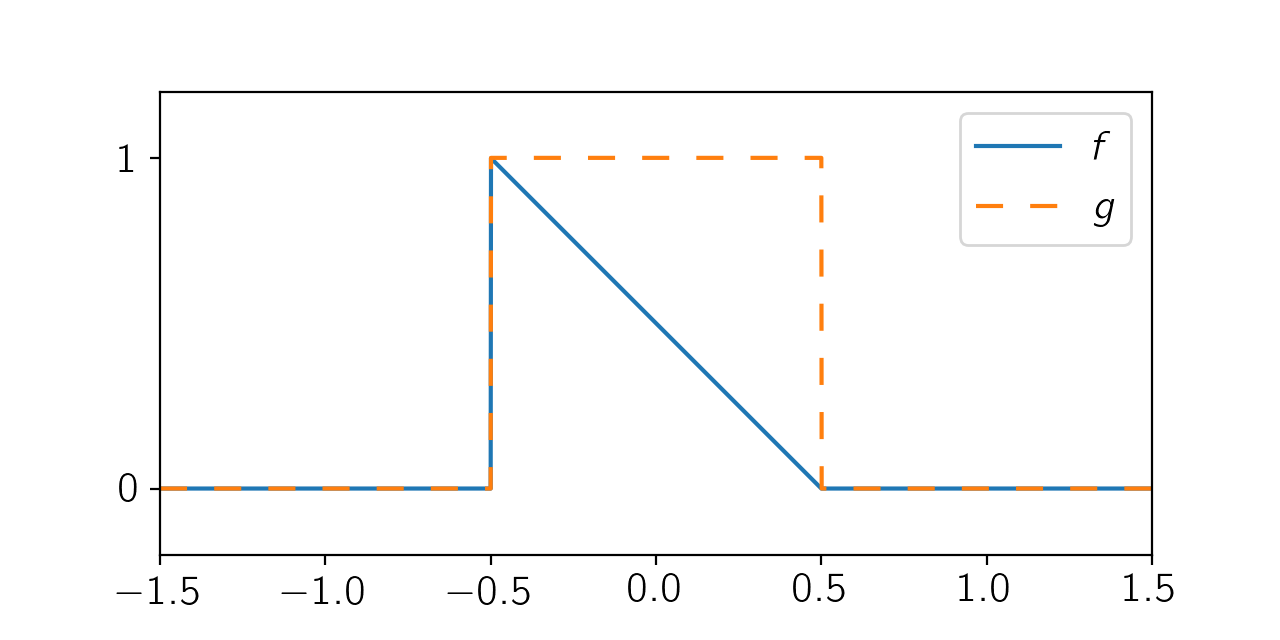
\includegraphics[width=\textwidth]{g.png}
    \end{subfigure}%
    \begin{subfigure}[c]{0.5\textwidth}
        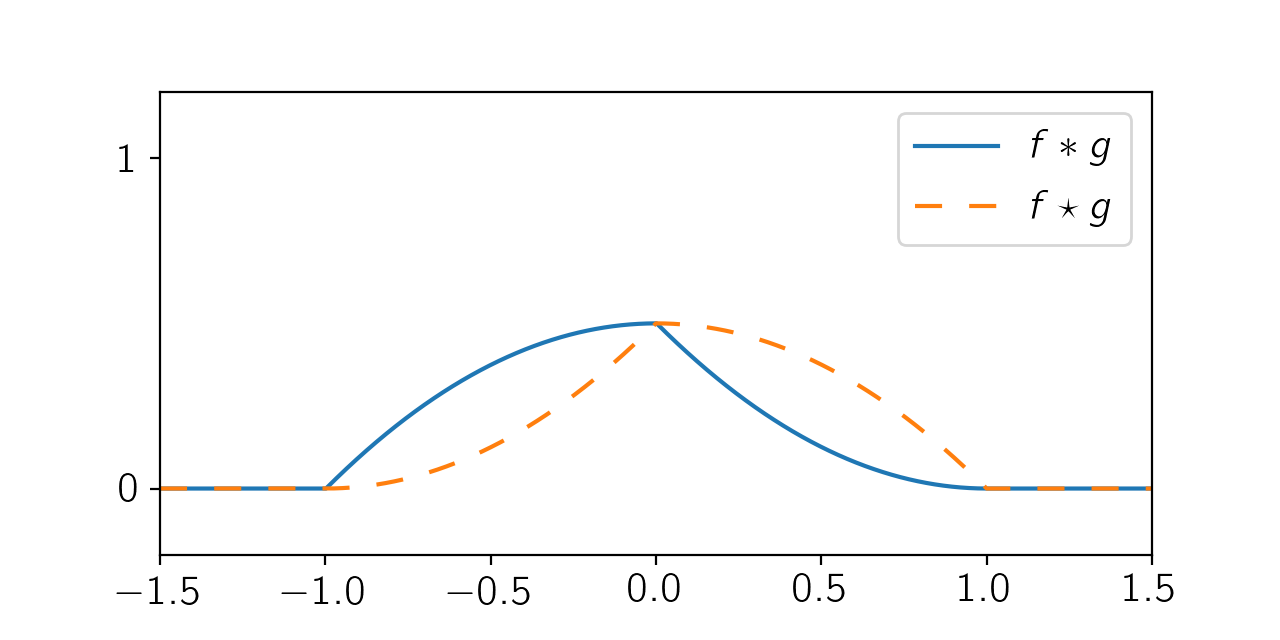
\includegraphics[width=\textwidth]{corrs.png}
    \end{subfigure}
    \caption{
        Die Kreuzkorrelation und Faltung von zwei kontinuierlichen, eindimensionalen Signalen.
    }
    \label{fig:one-dim-cont-conv}
\end{figure}


Wir stellen uns vor, dass der Graph von $f \star g$ durch das Schieben des Filters $f$ über das Signal $g$ von links nach rechts entsteht:
Dabei ist $(f\star g)(x)$ das Integral des Produktes der beiden Signale zu einem Zeitpunkt $x$, zu dem der Filter die Form $\tau \mapsto f(\tau - x)$ hat.
Hier entspricht dieses Integral gerade dem Flächeninhalt des Schnitts des verschobenen Dreieck-Filters mit dem Rechteck-Signal.
Die Faltung wird auf die gleiche Weise berechnet mit der Ausnahme, dass der Filter zunächst an der $y$-Achse gespiegelt wird.

\medskip

In Anwendungen werden meist diskrete Signale mit einem kompakten Träger betrachtet.
Ein diskretes Signal dieser Form schreiben wir im eindimensionalen Fall $d=1$ als Vektor $f = (f_0, f_1, \dots, f_{n-1})$, wobei wir für eine leichtere Notation stets bei $0$ anfangen zu indizieren.
Dazu führen wir als Notation $\fNat{n}\coloneqq \{0, \dots, n-1\}$ ein. 
Zweidimensionale Signale mit kompaktem Träger schreiben wir demnach als Matrix $F = (F_{i,j})_{i\in\fNat{m}, j\in\fNat{n}}$.
Diese Signale werden für Indizes außerhalb der so definierten Vektoren bzw. Matrizen als $0$ ausgewertet, also beispielsweise $f_z = 0$ für $z\in\Z\setminus\fNat{n}$ mit $f=(f_0, \dots, f_{n-1})$.

Als Beispiel betrachten wir die Kreuzkorrelation mit dem diskreten Filter $f=(\frac{1}{2}, \frac{1}{2})$.
Damit erhalten wir den sogenannten \emph{gleitenden Mittelwert} von einem Signal $g$:
\[  
    (f \star g)_i = \int_\Z f_\tau \cdot g_{i + \tau} \diff \cmeasure(\tau) 
    = \sum_{\tau\in\Z} f_\tau \cdot g_{i+ \tau}
    = \frac{g_i}{2} + \frac{g_{i+1}}{2} = \frac{g_i + g_{i+1}}{2}
\]

Auch die zweidimensionale Kreuzkorrelation lässt sich einfach veranschaulichen:
Grau\-stufen-Bilder werden oft als eine Matrix $G\in[0,1]^{r\times c}$ enkodiert, wobei $r$ die Anzahl an Reihen, $c$ die Anzahl an Spalten und ein Eintrag $G_{i,j}$ die \emph{Aktivierung des Pixels} zwischen~$0$ und~$1$ beschreiben.
Dabei stehen der Wert~$0$ für Schwarz und der Wert~$1$ für Weiß.
Für ein Beispiel eines zweidimensionalen Filters betrachten wir den sogenannten \emph{Sobel-Filter} zur Erkennung von horizontalen Kanten.
Dieser hat die Form
\[
    F = \begin{pmatrix}
        1 & 2 & 1 \\
        0 & 0 & 0 \\ 
        -1 & -2 & -1
    \end{pmatrix}.
\]


\begin{figure}
    \centering
    \begin{subfigure}{0.4\textwidth}
        \resizebox{\textwidth}{\textwidth}{
        \tikzset{ 
table/.style={
    matrix of nodes,
    nodes={rectangle,minimum size=0.05cm,align=center},
    nodes in empty cells
    }
}
\begin{tikzpicture}
    \matrix (mat) [table]
    {
    |[fill=white!0!black] | & |[fill=white!0!black] | & |[fill=white!0!black] | & |[fill=white!0!black] | & |[fill=white!0!black] | & |[fill=white!0!black] | & |[fill=white!0!black] | & |[fill=white!0!black] | & |[fill=white!0!black] | & |[fill=white!0!black] | & |[fill=white!0!black] | & |[fill=white!0!black] | & |[fill=white!0!black] | & |[fill=white!0!black] | & |[fill=white!0!black] | & |[fill=white!0!black] | & |[fill=white!0!black] | & |[fill=white!0!black] | & |[fill=white!0!black] | & |[fill=white!0!black] | & |[fill=white!0!black] | & |[fill=white!0!black] | & |[fill=white!0!black] | & |[fill=white!0!black] | & |[fill=white!0!black] | & |[fill=white!0!black] | & |[fill=white!0!black] | & |[fill=white!0!black] |\\
    |[fill=white!0!black] | & |[fill=white!0!black] | & |[fill=white!0!black] | & |[fill=white!0!black] | & |[fill=white!0!black] | & |[fill=white!0!black] | & |[fill=white!0!black] | & |[fill=white!0!black] | & |[fill=white!0!black] | & |[fill=white!0!black] | & |[fill=white!0!black] | & |[fill=white!0!black] | & |[fill=white!0!black] | & |[fill=white!0!black] | & |[fill=white!0!black] | & |[fill=white!0!black] | & |[fill=white!0!black] | & |[fill=white!0!black] | & |[fill=white!0!black] | & |[fill=white!0!black] | & |[fill=white!0!black] | & |[fill=white!0!black] | & |[fill=white!0!black] | & |[fill=white!0!black] | & |[fill=white!0!black] | & |[fill=white!0!black] | & |[fill=white!0!black] | & |[fill=white!0!black] |\\
    |[fill=white!0!black] | & |[fill=white!0!black] | & |[fill=white!0!black] | & |[fill=white!0!black] | & |[fill=white!0!black] | & |[fill=white!0!black] | & |[fill=white!0!black] | & |[fill=white!0!black] | & |[fill=white!0!black] | & |[fill=white!0!black] | & |[fill=white!0!black] | & |[fill=white!0!black] | & |[fill=white!0!black] | & |[fill=white!0!black] | & |[fill=white!0!black] | & |[fill=white!0!black] | & |[fill=white!0!black] | & |[fill=white!0!black] | & |[fill=white!0!black] | & |[fill=white!0!black] | & |[fill=white!0!black] | & |[fill=white!0!black] | & |[fill=white!0!black] | & |[fill=white!0!black] | & |[fill=white!0!black] | & |[fill=white!0!black] | & |[fill=white!0!black] | & |[fill=white!0!black] |\\
    |[fill=white!0!black] | & |[fill=white!0!black] | & |[fill=white!0!black] | & |[fill=white!0!black] | & |[fill=white!0!black] | & |[fill=white!0!black] | & |[fill=white!0!black] | & |[fill=white!0!black] | & |[fill=white!0!black] | & |[fill=white!0!black] | & |[fill=white!0!black] | & |[fill=white!0!black] | & |[fill=white!0!black] | & |[fill=white!0!black] | & |[fill=white!0!black] | & |[fill=white!0!black] | & |[fill=white!0!black] | & |[fill=white!0!black] | & |[fill=white!0!black] | & |[fill=white!0!black] | & |[fill=white!0!black] | & |[fill=white!0!black] | & |[fill=white!0!black] | & |[fill=white!0!black] | & |[fill=white!0!black] | & |[fill=white!0!black] | & |[fill=white!0!black] | & |[fill=white!0!black] |\\
    |[fill=white!0!black] | & |[fill=white!0!black] | & |[fill=white!0!black] | & |[fill=white!0!black] | & |[fill=white!0!black] | & |[fill=white!0!black] | & |[fill=white!0!black] | & |[fill=white!0!black] | & |[fill=white!0!black] | & |[fill=white!0!black] | & |[fill=white!0!black] | & |[fill=white!0!black] | & |[fill=white!0!black] | & |[fill=white!0!black] | & |[fill=white!0!black] | & |[fill=white!0!black] | & |[fill=white!0!black] | & |[fill=white!0!black] | & |[fill=white!0!black] | & |[fill=white!0!black] | & |[fill=white!0!black] | & |[fill=white!53!black] | & |[fill=white!81!black] | & |[fill=white!0!black] | & |[fill=white!0!black] | & |[fill=white!0!black] | & |[fill=white!0!black] | & |[fill=white!0!black] |\\
    |[fill=white!0!black] | & |[fill=white!0!black] | & |[fill=white!0!black] | & |[fill=white!0!black] | & |[fill=white!0!black] | & |[fill=white!0!black] | & |[fill=white!0!black] | & |[fill=white!0!black] | & |[fill=white!0!black] | & |[fill=white!0!black] | & |[fill=white!0!black] | & |[fill=white!0!black] | & |[fill=white!0!black] | & |[fill=white!0!black] | & |[fill=white!0!black] | & |[fill=white!0!black] | & |[fill=white!0!black] | & |[fill=white!0!black] | & |[fill=white!0!black] | & |[fill=white!0!black] | & |[fill=white!27!black] | & |[fill=white!93!black] | & |[fill=white!81!black] | & |[fill=white!0!black] | & |[fill=white!0!black] | & |[fill=white!0!black] | & |[fill=white!0!black] | & |[fill=white!0!black] |\\
    |[fill=white!0!black] | & |[fill=white!0!black] | & |[fill=white!0!black] | & |[fill=white!0!black] | & |[fill=white!0!black] | & |[fill=white!0!black] | & |[fill=white!0!black] | & |[fill=white!0!black] | & |[fill=white!0!black] | & |[fill=white!0!black] | & |[fill=white!0!black] | & |[fill=white!0!black] | & |[fill=white!0!black] | & |[fill=white!0!black] | & |[fill=white!0!black] | & |[fill=white!0!black] | & |[fill=white!0!black] | & |[fill=white!0!black] | & |[fill=white!0!black] | & |[fill=white!1!black] | & |[fill=white!75!black] | & |[fill=white!100!black] | & |[fill=white!78!black] | & |[fill=white!0!black] | & |[fill=white!0!black] | & |[fill=white!0!black] | & |[fill=white!0!black] | & |[fill=white!0!black] |\\
    |[fill=white!0!black] | & |[fill=white!0!black] | & |[fill=white!0!black] | & |[fill=white!0!black] | & |[fill=white!0!black] | & |[fill=white!0!black] | & |[fill=white!0!black] | & |[fill=white!0!black] | & |[fill=white!0!black] | & |[fill=white!0!black] | & |[fill=white!0!black] | & |[fill=white!0!black] | & |[fill=white!0!black] | & |[fill=white!0!black] | & |[fill=white!0!black] | & |[fill=white!0!black] | & |[fill=white!0!black] | & |[fill=white!0!black] | & |[fill=white!0!black] | & |[fill=white!22!black] | & |[fill=white!99!black] | & |[fill=white!100!black] | & |[fill=white!19!black] | & |[fill=white!0!black] | & |[fill=white!0!black] | & |[fill=white!0!black] | & |[fill=white!0!black] | & |[fill=white!0!black] |\\
    |[fill=white!0!black] | & |[fill=white!0!black] | & |[fill=white!0!black] | & |[fill=white!0!black] | & |[fill=white!0!black] | & |[fill=white!0!black] | & |[fill=white!0!black] | & |[fill=white!0!black] | & |[fill=white!0!black] | & |[fill=white!0!black] | & |[fill=white!0!black] | & |[fill=white!0!black] | & |[fill=white!0!black] | & |[fill=white!0!black] | & |[fill=white!0!black] | & |[fill=white!0!black] | & |[fill=white!0!black] | & |[fill=white!0!black] | & |[fill=white!5!black] | & |[fill=white!73!black] | & |[fill=white!100!black] | & |[fill=white!82!black] | & |[fill=white!4!black] | & |[fill=white!0!black] | & |[fill=white!0!black] | & |[fill=white!0!black] | & |[fill=white!0!black] | & |[fill=white!0!black] |\\
    |[fill=white!0!black] | & |[fill=white!0!black] | & |[fill=white!0!black] | & |[fill=white!0!black] | & |[fill=white!0!black] | & |[fill=white!0!black] | & |[fill=white!0!black] | & |[fill=white!0!black] | & |[fill=white!0!black] | & |[fill=white!0!black] | & |[fill=white!0!black] | & |[fill=white!0!black] | & |[fill=white!0!black] | & |[fill=white!0!black] | & |[fill=white!0!black] | & |[fill=white!0!black] | & |[fill=white!0!black] | & |[fill=white!0!black] | & |[fill=white!38!black] | & |[fill=white!99!black] | & |[fill=white!86!black] | & |[fill=white!20!black] | & |[fill=white!0!black] | & |[fill=white!0!black] | & |[fill=white!0!black] | & |[fill=white!0!black] | & |[fill=white!0!black] | & |[fill=white!0!black] |\\
    |[fill=white!0!black] | & |[fill=white!0!black] | & |[fill=white!0!black] | & |[fill=white!0!black] | & |[fill=white!0!black] | & |[fill=white!0!black] | & |[fill=white!0!black] | & |[fill=white!0!black] | & |[fill=white!0!black] | & |[fill=white!0!black] | & |[fill=white!0!black] | & |[fill=white!0!black] | & |[fill=white!7!black] | & |[fill=white!22!black] | & |[fill=white!1!black] | & |[fill=white!0!black] | & |[fill=white!0!black] | & |[fill=white!26!black] | & |[fill=white!88!black] | & |[fill=white!99!black] | & |[fill=white!53!black] | & |[fill=white!0!black] | & |[fill=white!0!black] | & |[fill=white!0!black] | & |[fill=white!0!black] | & |[fill=white!0!black] | & |[fill=white!0!black] | & |[fill=white!0!black] |\\
    |[fill=white!0!black] | & |[fill=white!0!black] | & |[fill=white!0!black] | & |[fill=white!0!black] | & |[fill=white!0!black] | & |[fill=white!0!black] | & |[fill=white!0!black] | & |[fill=white!0!black] | & |[fill=white!0!black] | & |[fill=white!0!black] | & |[fill=white!0!black] | & |[fill=white!33!black] | & |[fill=white!92!black] | & |[fill=white!89!black] | & |[fill=white!6!black] | & |[fill=white!0!black] | & |[fill=white!0!black] | & |[fill=white!53!black] | & |[fill=white!99!black] | & |[fill=white!79!black] | & |[fill=white!7!black] | & |[fill=white!0!black] | & |[fill=white!0!black] | & |[fill=white!0!black] | & |[fill=white!0!black] | & |[fill=white!0!black] | & |[fill=white!0!black] | & |[fill=white!0!black] |\\
    |[fill=white!0!black] | & |[fill=white!0!black] | & |[fill=white!0!black] | & |[fill=white!0!black] | & |[fill=white!0!black] | & |[fill=white!0!black] | & |[fill=white!0!black] | & |[fill=white!0!black] | & |[fill=white!0!black] | & |[fill=white!0!black] | & |[fill=white!0!black] | & |[fill=white!36!black] | & |[fill=white!100!black] | & |[fill=white!59!black] | & |[fill=white!4!black] | & |[fill=white!0!black] | & |[fill=white!36!black] | & |[fill=white!100!black] | & |[fill=white!100!black] | & |[fill=white!44!black] | & |[fill=white!0!black] | & |[fill=white!0!black] | & |[fill=white!0!black] | & |[fill=white!0!black] | & |[fill=white!0!black] | & |[fill=white!0!black] | & |[fill=white!0!black] | & |[fill=white!0!black] |\\
    |[fill=white!0!black] | & |[fill=white!0!black] | & |[fill=white!0!black] | & |[fill=white!0!black] | & |[fill=white!0!black] | & |[fill=white!0!black] | & |[fill=white!0!black] | & |[fill=white!0!black] | & |[fill=white!0!black] | & |[fill=white!0!black] | & |[fill=white!0!black] | & |[fill=white!1!black] | & |[fill=white!35!black] | & |[fill=white!16!black] | & |[fill=white!0!black] | & |[fill=white!12!black] | & |[fill=white!84!black] | & |[fill=white!100!black] | & |[fill=white!63!black] | & |[fill=white!2!black] | & |[fill=white!0!black] | & |[fill=white!0!black] | & |[fill=white!0!black] | & |[fill=white!0!black] | & |[fill=white!0!black] | & |[fill=white!0!black] | & |[fill=white!0!black] | & |[fill=white!0!black] |\\
    |[fill=white!0!black] | & |[fill=white!0!black] | & |[fill=white!0!black] | & |[fill=white!0!black] | & |[fill=white!0!black] | & |[fill=white!0!black] | & |[fill=white!0!black] | & |[fill=white!0!black] | & |[fill=white!0!black] | & |[fill=white!29!black] | & |[fill=white!81!black] | & |[fill=white!65!black] | & |[fill=white!13!black] | & |[fill=white!0!black] | & |[fill=white!0!black] | & |[fill=white!62!black] | & |[fill=white!99!black] | & |[fill=white!77!black] | & |[fill=white!8!black] | & |[fill=white!0!black] | & |[fill=white!0!black] | & |[fill=white!0!black] | & |[fill=white!0!black] | & |[fill=white!0!black] | & |[fill=white!0!black] | & |[fill=white!0!black] | & |[fill=white!0!black] | & |[fill=white!0!black] |\\
    |[fill=white!0!black] | & |[fill=white!0!black] | & |[fill=white!0!black] | & |[fill=white!0!black] | & |[fill=white!0!black] | & |[fill=white!0!black] | & |[fill=white!0!black] | & |[fill=white!0!black] | & |[fill=white!27!black] | & |[fill=white!86!black] | & |[fill=white!99!black] | & |[fill=white!82!black] | & |[fill=white!17!black] | & |[fill=white!0!black] | & |[fill=white!20!black] | & |[fill=white!88!black] | & |[fill=white!86!black] | & |[fill=white!46!black] | & |[fill=white!0!black] | & |[fill=white!0!black] | & |[fill=white!0!black] | & |[fill=white!0!black] | & |[fill=white!0!black] | & |[fill=white!0!black] | & |[fill=white!0!black] | & |[fill=white!0!black] | & |[fill=white!0!black] | & |[fill=white!0!black] |\\
    |[fill=white!0!black] | & |[fill=white!0!black] | & |[fill=white!0!black] | & |[fill=white!0!black] | & |[fill=white!0!black] | & |[fill=white!0!black] | & |[fill=white!0!black] | & |[fill=white!16!black] | & |[fill=white!90!black] | & |[fill=white!100!black] | & |[fill=white!75!black] | & |[fill=white!13!black] | & |[fill=white!0!black] | & |[fill=white!0!black] | & |[fill=white!51!black] | & |[fill=white!100!black] | & |[fill=white!66!black] | & |[fill=white!0!black] | & |[fill=white!0!black] | & |[fill=white!0!black] | & |[fill=white!0!black] | & |[fill=white!0!black] | & |[fill=white!0!black] | & |[fill=white!0!black] | & |[fill=white!0!black] | & |[fill=white!0!black] | & |[fill=white!0!black] | & |[fill=white!0!black] |\\
    |[fill=white!0!black] | & |[fill=white!0!black] | & |[fill=white!0!black] | & |[fill=white!0!black] | & |[fill=white!0!black] | & |[fill=white!0!black] | & |[fill=white!10!black] | & |[fill=white!88!black] | & |[fill=white!99!black] | & |[fill=white!100!black] | & |[fill=white!25!black] | & |[fill=white!35!black] | & |[fill=white!54!black] | & |[fill=white!64!black] | & |[fill=white!98!black] | & |[fill=white!99!black] | & |[fill=white!66!black] | & |[fill=white!55!black] | & |[fill=white!64!black] | & |[fill=white!40!black] | & |[fill=white!0!black] | & |[fill=white!0!black] | & |[fill=white!0!black] | & |[fill=white!0!black] | & |[fill=white!0!black] | & |[fill=white!0!black] | & |[fill=white!0!black] | & |[fill=white!0!black] |\\
    |[fill=white!0!black] | & |[fill=white!0!black] | & |[fill=white!0!black] | & |[fill=white!0!black] | & |[fill=white!0!black] | & |[fill=white!0!black] | & |[fill=white!10!black] | & |[fill=white!91!black] | & |[fill=white!99!black] | & |[fill=white!100!black] | & |[fill=white!99!black] | & |[fill=white!99!black] | & |[fill=white!99!black] | & |[fill=white!100!black] | & |[fill=white!99!black] | & |[fill=white!92!black] | & |[fill=white!77!black] | & |[fill=white!54!black] | & |[fill=white!25!black] | & |[fill=white!0!black] | & |[fill=white!0!black] | & |[fill=white!0!black] | & |[fill=white!0!black] | & |[fill=white!0!black] | & |[fill=white!0!black] | & |[fill=white!0!black] | & |[fill=white!0!black] | & |[fill=white!0!black] |\\
    |[fill=white!0!black] | & |[fill=white!0!black] | & |[fill=white!0!black] | & |[fill=white!0!black] | & |[fill=white!0!black] | & |[fill=white!0!black] | & |[fill=white!0!black] | & |[fill=white!25!black] | & |[fill=white!37!black] | & |[fill=white!50!black] | & |[fill=white!63!black] | & |[fill=white!66!black] | & |[fill=white!99!black] | & |[fill=white!100!black] | & |[fill=white!59!black] | & |[fill=white!5!black] | & |[fill=white!0!black] | & |[fill=white!0!black] | & |[fill=white!0!black] | & |[fill=white!0!black] | & |[fill=white!0!black] | & |[fill=white!0!black] | & |[fill=white!0!black] | & |[fill=white!0!black] | & |[fill=white!0!black] | & |[fill=white!0!black] | & |[fill=white!0!black] | & |[fill=white!0!black] |\\
    |[fill=white!0!black] | & |[fill=white!0!black] | & |[fill=white!0!black] | & |[fill=white!0!black] | & |[fill=white!0!black] | & |[fill=white!0!black] | & |[fill=white!0!black] | & |[fill=white!0!black] | & |[fill=white!0!black] | & |[fill=white!0!black] | & |[fill=white!0!black] | & |[fill=white!55!black] | & |[fill=white!100!black] | & |[fill=white!63!black] | & |[fill=white!0!black] | & |[fill=white!0!black] | & |[fill=white!0!black] | & |[fill=white!0!black] | & |[fill=white!0!black] | & |[fill=white!0!black] | & |[fill=white!0!black] | & |[fill=white!0!black] | & |[fill=white!0!black] | & |[fill=white!0!black] | & |[fill=white!0!black] | & |[fill=white!0!black] | & |[fill=white!0!black] | & |[fill=white!0!black] |\\
    |[fill=white!0!black] | & |[fill=white!0!black] | & |[fill=white!0!black] | & |[fill=white!0!black] | & |[fill=white!0!black] | & |[fill=white!0!black] | & |[fill=white!0!black] | & |[fill=white!0!black] | & |[fill=white!0!black] | & |[fill=white!0!black] | & |[fill=white!17!black] | & |[fill=white!91!black] | & |[fill=white!86!black] | & |[fill=white!4!black] | & |[fill=white!0!black] | & |[fill=white!0!black] | & |[fill=white!0!black] | & |[fill=white!0!black] | & |[fill=white!0!black] | & |[fill=white!0!black] | & |[fill=white!0!black] | & |[fill=white!0!black] | & |[fill=white!0!black] | & |[fill=white!0!black] | & |[fill=white!0!black] | & |[fill=white!0!black] | & |[fill=white!0!black] | & |[fill=white!0!black] |\\
    |[fill=white!0!black] | & |[fill=white!0!black] | & |[fill=white!0!black] | & |[fill=white!0!black] | & |[fill=white!0!black] | & |[fill=white!0!black] | & |[fill=white!0!black] | & |[fill=white!0!black] | & |[fill=white!0!black] | & |[fill=white!0!black] | & |[fill=white!71!black] | & |[fill=white!99!black] | & |[fill=white!27!black] | & |[fill=white!0!black] | & |[fill=white!0!black] | & |[fill=white!0!black] | & |[fill=white!0!black] | & |[fill=white!0!black] | & |[fill=white!0!black] | & |[fill=white!0!black] | & |[fill=white!0!black] | & |[fill=white!0!black] | & |[fill=white!0!black] | & |[fill=white!0!black] | & |[fill=white!0!black] | & |[fill=white!0!black] | & |[fill=white!0!black] | & |[fill=white!0!black] |\\
    |[fill=white!0!black] | & |[fill=white!0!black] | & |[fill=white!0!black] | & |[fill=white!0!black] | & |[fill=white!0!black] | & |[fill=white!0!black] | & |[fill=white!0!black] | & |[fill=white!0!black] | & |[fill=white!0!black] | & |[fill=white!0!black] | & |[fill=white!64!black] | & |[fill=white!96!black] | & |[fill=white!31!black] | & |[fill=white!0!black] | & |[fill=white!0!black] | & |[fill=white!0!black] | & |[fill=white!0!black] | & |[fill=white!0!black] | & |[fill=white!0!black] | & |[fill=white!0!black] | & |[fill=white!0!black] | & |[fill=white!0!black] | & |[fill=white!0!black] | & |[fill=white!0!black] | & |[fill=white!0!black] | & |[fill=white!0!black] | & |[fill=white!0!black] | & |[fill=white!0!black] |\\
    |[fill=white!0!black] | & |[fill=white!0!black] | & |[fill=white!0!black] | & |[fill=white!0!black] | & |[fill=white!0!black] | & |[fill=white!0!black] | & |[fill=white!0!black] | & |[fill=white!0!black] | & |[fill=white!0!black] | & |[fill=white!0!black] | & |[fill=white!0!black] | & |[fill=white!0!black] | & |[fill=white!0!black] | & |[fill=white!0!black] | & |[fill=white!0!black] | & |[fill=white!0!black] | & |[fill=white!0!black] | & |[fill=white!0!black] | & |[fill=white!0!black] | & |[fill=white!0!black] | & |[fill=white!0!black] | & |[fill=white!0!black] | & |[fill=white!0!black] | & |[fill=white!0!black] | & |[fill=white!0!black] | & |[fill=white!0!black] | & |[fill=white!0!black] | & |[fill=white!0!black] |\\
    |[fill=white!0!black] | & |[fill=white!0!black] | & |[fill=white!0!black] | & |[fill=white!0!black] | & |[fill=white!0!black] | & |[fill=white!0!black] | & |[fill=white!0!black] | & |[fill=white!0!black] | & |[fill=white!0!black] | & |[fill=white!0!black] | & |[fill=white!0!black] | & |[fill=white!0!black] | & |[fill=white!0!black] | & |[fill=white!0!black] | & |[fill=white!0!black] | & |[fill=white!0!black] | & |[fill=white!0!black] | & |[fill=white!0!black] | & |[fill=white!0!black] | & |[fill=white!0!black] | & |[fill=white!0!black] | & |[fill=white!0!black] | & |[fill=white!0!black] | & |[fill=white!0!black] | & |[fill=white!0!black] | & |[fill=white!0!black] | & |[fill=white!0!black] | & |[fill=white!0!black] |\\
    |[fill=white!0!black] | & |[fill=white!0!black] | & |[fill=white!0!black] | & |[fill=white!0!black] | & |[fill=white!0!black] | & |[fill=white!0!black] | & |[fill=white!0!black] | & |[fill=white!0!black] | & |[fill=white!0!black] | & |[fill=white!0!black] | & |[fill=white!0!black] | & |[fill=white!0!black] | & |[fill=white!0!black] | & |[fill=white!0!black] | & |[fill=white!0!black] | & |[fill=white!0!black] | & |[fill=white!0!black] | & |[fill=white!0!black] | & |[fill=white!0!black] | & |[fill=white!0!black] | & |[fill=white!0!black] | & |[fill=white!0!black] | & |[fill=white!0!black] | & |[fill=white!0!black] | & |[fill=white!0!black] | & |[fill=white!0!black] | & |[fill=white!0!black] | & |[fill=white!0!black] |\\
    |[fill=white!0!black] | & |[fill=white!0!black] | & |[fill=white!0!black] | & |[fill=white!0!black] | & |[fill=white!0!black] | & |[fill=white!0!black] | & |[fill=white!0!black] | & |[fill=white!0!black] | & |[fill=white!0!black] | & |[fill=white!0!black] | & |[fill=white!0!black] | & |[fill=white!0!black] | & |[fill=white!0!black] | & |[fill=white!0!black] | & |[fill=white!0!black] | & |[fill=white!0!black] | & |[fill=white!0!black] | & |[fill=white!0!black] | & |[fill=white!0!black] | & |[fill=white!0!black] | & |[fill=white!0!black] | & |[fill=white!0!black] | & |[fill=white!0!black] | & |[fill=white!0!black] | & |[fill=white!0!black] | & |[fill=white!0!black] | & |[fill=white!0!black] | & |[fill=white!0!black] |\\
    };
\end{tikzpicture}
        }
        \caption{Das Input-Signal $G$.\\Schwarz $\hat=$ $0$, Weiß $\hat=$ $1$.}
    \end{subfigure}%
    \begin{subfigure}{0.4\textwidth}
        \resizebox{0.9285\textwidth}{0.9285\textwidth}{
        
\tikzset{ 
table/.style={
    matrix of nodes,
    nodes={rectangle,minimum size=0.05cm,align=center},
    nodes in empty cells
    }
}
\begin{tikzpicture}
    \matrix (mat) [table]
    {
    |[fill=white!0!black] | & |[fill=white!0!black] | & |[fill=white!0!black] | & |[fill=white!0!black] | & |[fill=white!0!black] | & |[fill=white!0!black] | & |[fill=white!0!black] | & |[fill=white!0!black] | & |[fill=white!0!black] | & |[fill=white!0!black] | & |[fill=white!0!black] | & |[fill=white!0!black] | & |[fill=white!0!black] | & |[fill=white!0!black] | & |[fill=white!0!black] | & |[fill=white!0!black] | & |[fill=white!0!black] | & |[fill=white!0!black] | & |[fill=white!0!black] | & |[fill=white!0!black] | & |[fill=white!0!black] | & |[fill=white!0!black] | & |[fill=white!0!black] | & |[fill=white!0!black] | & |[fill=white!0!black] | & |[fill=white!0!black] | & |[fill=white!0!black] | & |[fill=white!0!black] |\\
    |[fill=white!0!black] | & |[fill=white!0!black] | & |[fill=white!0!black] | & |[fill=white!0!black] | & |[fill=white!0!black] | & |[fill=white!0!black] | & |[fill=white!0!black] | & |[fill=white!0!black] | & |[fill=white!0!black] | & |[fill=white!0!black] | & |[fill=white!0!black] | & |[fill=white!0!black] | & |[fill=white!0!black] | & |[fill=white!0!black] | & |[fill=white!0!black] | & |[fill=white!0!black] | & |[fill=white!0!black] | & |[fill=white!0!black] | & |[fill=white!0!black] | & |[fill=white!0!black] | & |[fill=white!0!black] | & |[fill=white!0!black] | & |[fill=white!0!black] | & |[fill=white!0!black] | & |[fill=white!0!black] | & |[fill=white!0!black] | & |[fill=white!0!black] | & |[fill=white!0!black] |\\
    |[fill=white!0!black] | & |[fill=white!0!black] | & |[fill=white!0!black] | & |[fill=white!0!black] | & |[fill=white!0!black] | & |[fill=white!0!black] | & |[fill=white!0!black] | & |[fill=white!0!black] | & |[fill=white!0!black] | & |[fill=white!0!black] | & |[fill=white!0!black] | & |[fill=white!0!black] | & |[fill=white!0!black] | & |[fill=white!0!black] | & |[fill=white!0!black] | & |[fill=white!0!black] | & |[fill=white!0!black] | & |[fill=white!0!black] | & |[fill=white!0!black] | & |[fill=white!0!black] | & |[fill=white!0!black] | & |[fill=white!0!black] | & |[fill=white!0!black] | & |[fill=white!0!black] | & |[fill=white!0!black] | & |[fill=white!0!black] | & |[fill=white!0!black] | & |[fill=white!0!black] |\\
    |[fill=white!0!black] | & |[fill=white!0!black] | & |[fill=white!0!black] | & |[fill=white!0!black] | & |[fill=white!0!black] | & |[fill=white!0!black] | & |[fill=white!0!black] | & |[fill=white!0!black] | & |[fill=white!0!black] | & |[fill=white!0!black] | & |[fill=white!0!black] | & |[fill=white!0!black] | & |[fill=white!0!black] | & |[fill=white!0!black] | & |[fill=white!0!black] | & |[fill=white!0!black] | & |[fill=white!0!black] | & |[fill=white!0!black] | & |[fill=white!0!black] | & |[fill=white!0!black] | & |[fill=white!0!black] | & |[fill=white!0!black] | & |[fill=white!0!black] | & |[fill=white!0!black] | & |[fill=white!0!black] | & |[fill=white!0!black] | & |[fill=white!0!black] | & |[fill=white!0!black] |\\
    |[fill=white!0!black] | & |[fill=white!0!black] | & |[fill=white!0!black] | & |[fill=white!0!black] | & |[fill=white!0!black] | & |[fill=white!0!black] | & |[fill=white!0!black] | & |[fill=white!0!black] | & |[fill=white!0!black] | & |[fill=white!0!black] | & |[fill=white!0!black] | & |[fill=white!0!black] | & |[fill=white!0!black] | & |[fill=white!0!black] | & |[fill=white!0!black] | & |[fill=white!0!black] | & |[fill=white!0!black] | & |[fill=white!0!black] | & |[fill=white!0!black] | & |[fill=white!0!black] | & |[fill=white!0!black] | & |[fill=white!0!black] | & |[fill=white!0!black] | & |[fill=white!0!black] | & |[fill=white!0!black] | & |[fill=white!0!black] | & |[fill=white!0!black] | & |[fill=white!0!black] |\\
    |[fill=white!0!black] | & |[fill=white!0!black] | & |[fill=white!0!black] | & |[fill=white!0!black] | & |[fill=white!0!black] | & |[fill=white!0!black] | & |[fill=white!0!black] | & |[fill=white!0!black] | & |[fill=white!0!black] | & |[fill=white!0!black] | & |[fill=white!0!black] | & |[fill=white!0!black] | & |[fill=white!0!black] | & |[fill=white!0!black] | & |[fill=white!0!black] | & |[fill=white!0!black] | & |[fill=white!0!black] | & |[fill=white!0!black] | & |[fill=white!0!black] | & |[fill=white!0!black] | & |[fill=white!0!black] | & |[fill=white!0!black] | & |[fill=white!0!black] | & |[fill=white!3!black] | & |[fill=white!0!black] | & |[fill=white!0!black] | & |[fill=white!0!black] | & |[fill=white!0!black] |\\
    |[fill=white!0!black] | & |[fill=white!0!black] | & |[fill=white!0!black] | & |[fill=white!0!black] | & |[fill=white!0!black] | & |[fill=white!0!black] | & |[fill=white!0!black] | & |[fill=white!0!black] | & |[fill=white!0!black] | & |[fill=white!0!black] | & |[fill=white!0!black] | & |[fill=white!0!black] | & |[fill=white!0!black] | & |[fill=white!0!black] | & |[fill=white!0!black] | & |[fill=white!0!black] | & |[fill=white!0!black] | & |[fill=white!0!black] | & |[fill=white!0!black] | & |[fill=white!0!black] | & |[fill=white!0!black] | & |[fill=white!0!black] | & |[fill=white!47!black] | & |[fill=white!53!black] | & |[fill=white!0!black] | & |[fill=white!0!black] | & |[fill=white!0!black] | & |[fill=white!0!black] |\\
    |[fill=white!0!black] | & |[fill=white!0!black] | & |[fill=white!0!black] | & |[fill=white!0!black] | & |[fill=white!0!black] | & |[fill=white!0!black] | & |[fill=white!0!black] | & |[fill=white!0!black] | & |[fill=white!0!black] | & |[fill=white!0!black] | & |[fill=white!0!black] | & |[fill=white!0!black] | & |[fill=white!0!black] | & |[fill=white!0!black] | & |[fill=white!0!black] | & |[fill=white!0!black] | & |[fill=white!0!black] | & |[fill=white!0!black] | & |[fill=white!0!black] | & |[fill=white!0!black] | & |[fill=white!0!black] | & |[fill=white!57!black] | & |[fill=white!78!black] | & |[fill=white!63!black] | & |[fill=white!0!black] | & |[fill=white!0!black] | & |[fill=white!0!black] | & |[fill=white!0!black] |\\
    |[fill=white!0!black] | & |[fill=white!0!black] | & |[fill=white!0!black] | & |[fill=white!0!black] | & |[fill=white!0!black] | & |[fill=white!0!black] | & |[fill=white!0!black] | & |[fill=white!0!black] | & |[fill=white!0!black] | & |[fill=white!0!black] | & |[fill=white!0!black] | & |[fill=white!0!black] | & |[fill=white!0!black] | & |[fill=white!0!black] | & |[fill=white!0!black] | & |[fill=white!0!black] | & |[fill=white!0!black] | & |[fill=white!0!black] | & |[fill=white!0!black] | & |[fill=white!0!black] | & |[fill=white!14!black] | & |[fill=white!95!black] | & |[fill=white!84!black] | & |[fill=white!16!black] | & |[fill=white!0!black] | & |[fill=white!0!black] | & |[fill=white!0!black] | & |[fill=white!0!black] |\\
    |[fill=white!0!black] | & |[fill=white!0!black] | & |[fill=white!0!black] | & |[fill=white!0!black] | & |[fill=white!0!black] | & |[fill=white!0!black] | & |[fill=white!0!black] | & |[fill=white!0!black] | & |[fill=white!0!black] | & |[fill=white!0!black] | & |[fill=white!0!black] | & |[fill=white!0!black] | & |[fill=white!0!black] | & |[fill=white!0!black] | & |[fill=white!0!black] | & |[fill=white!0!black] | & |[fill=white!0!black] | & |[fill=white!0!black] | & |[fill=white!0!black] | & |[fill=white!0!black] | & |[fill=white!88!black] | & |[fill=white!113!black] | & |[fill=white!73!black] | & |[fill=white!3!black] | & |[fill=white!0!black] | & |[fill=white!0!black] | & |[fill=white!0!black] | & |[fill=white!0!black] |\\
    |[fill=white!0!black] | & |[fill=white!0!black] | & |[fill=white!0!black] | & |[fill=white!0!black] | & |[fill=white!0!black] | & |[fill=white!0!black] | & |[fill=white!0!black] | & |[fill=white!0!black] | & |[fill=white!0!black] | & |[fill=white!0!black] | & |[fill=white!0!black] | & |[fill=white!0!black] | & |[fill=white!0!black] | & |[fill=white!0!black] | & |[fill=white!0!black] | & |[fill=white!0!black] | & |[fill=white!0!black] | & |[fill=white!0!black] | & |[fill=white!0!black] | & |[fill=white!32!black] | & |[fill=white!100!black] | & |[fill=white!83!black] | & |[fill=white!17!black] | & |[fill=white!0!black] | & |[fill=white!0!black] | & |[fill=white!0!black] | & |[fill=white!0!black] | & |[fill=white!0!black] |\\
    |[fill=white!0!black] | & |[fill=white!0!black] | & |[fill=white!0!black] | & |[fill=white!0!black] | & |[fill=white!0!black] | & |[fill=white!0!black] | & |[fill=white!0!black] | & |[fill=white!0!black] | & |[fill=white!0!black] | & |[fill=white!0!black] | & |[fill=white!0!black] | & |[fill=white!0!black] | & |[fill=white!0!black] | & |[fill=white!0!black] | & |[fill=white!0!black] | & |[fill=white!0!black] | & |[fill=white!0!black] | & |[fill=white!0!black] | & |[fill=white!0!black] | & |[fill=white!82!black] | & |[fill=white!92!black] | & |[fill=white!45!black] | & |[fill=white!0!black] | & |[fill=white!0!black] | & |[fill=white!0!black] | & |[fill=white!0!black] | & |[fill=white!0!black] | & |[fill=white!0!black] |\\
    |[fill=white!0!black] | & |[fill=white!0!black] | & |[fill=white!0!black] | & |[fill=white!0!black] | & |[fill=white!0!black] | & |[fill=white!0!black] | & |[fill=white!0!black] | & |[fill=white!0!black] | & |[fill=white!0!black] | & |[fill=white!0!black] | & |[fill=white!27!black] | & |[fill=white!75!black] | & |[fill=white!137!black] | & |[fill=white!115!black] | & |[fill=white!57!black] | & |[fill=white!0!black] | & |[fill=white!0!black] | & |[fill=white!0!black] | & |[fill=white!58!black] | & |[fill=white!103!black] | & |[fill=white!72!black] | & |[fill=white!6!black] | & |[fill=white!0!black] | & |[fill=white!0!black] | & |[fill=white!0!black] | & |[fill=white!0!black] | & |[fill=white!0!black] | & |[fill=white!0!black] |\\
    |[fill=white!0!black] | & |[fill=white!0!black] | & |[fill=white!0!black] | & |[fill=white!0!black] | & |[fill=white!0!black] | & |[fill=white!0!black] | & |[fill=white!0!black] | & |[fill=white!0!black] | & |[fill=white!0!black] | & |[fill=white!0!black] | & |[fill=white!0!black] | & |[fill=white!0!black] | & |[fill=white!100!black] | & |[fill=white!127!black] | & |[fill=white!1!black] | & |[fill=white!0!black] | & |[fill=white!0!black] | & |[fill=white!43!black] | & |[fill=white!134!black] | & |[fill=white!115!black] | & |[fill=white!38!black] | & |[fill=white!0!black] | & |[fill=white!0!black] | & |[fill=white!0!black] | & |[fill=white!0!black] | & |[fill=white!0!black] | & |[fill=white!0!black] | & |[fill=white!0!black] |\\
    |[fill=white!0!black] | & |[fill=white!0!black] | & |[fill=white!0!black] | & |[fill=white!0!black] | & |[fill=white!0!black] | & |[fill=white!0!black] | & |[fill=white!0!black] | & |[fill=white!0!black] | & |[fill=white!0!black] | & |[fill=white!0!black] | & |[fill=white!0!black] | & |[fill=white!0!black] | & |[fill=white!0!black] | & |[fill=white!12!black] | & |[fill=white!0!black] | & |[fill=white!0!black] | & |[fill=white!0!black] | & |[fill=white!97!black] | & |[fill=white!100!black] | & |[fill=white!55!black] | & |[fill=white!1!black] | & |[fill=white!0!black] | & |[fill=white!0!black] | & |[fill=white!0!black] | & |[fill=white!0!black] | & |[fill=white!0!black] | & |[fill=white!0!black] | & |[fill=white!0!black] |\\
    |[fill=white!0!black] | & |[fill=white!0!black] | & |[fill=white!0!black] | & |[fill=white!0!black] | & |[fill=white!0!black] | & |[fill=white!0!black] | & |[fill=white!0!black] | & |[fill=white!0!black] | & |[fill=white!0!black] | & |[fill=white!0!black] | & |[fill=white!0!black] | & |[fill=white!60!black] | & |[fill=white!54!black] | & |[fill=white!0!black] | & |[fill=white!0!black] | & |[fill=white!0!black] | & |[fill=white!61!black] | & |[fill=white!101!black] | & |[fill=white!73!black] | & |[fill=white!7!black] | & |[fill=white!0!black] | & |[fill=white!0!black] | & |[fill=white!0!black] | & |[fill=white!0!black] | & |[fill=white!0!black] | & |[fill=white!0!black] | & |[fill=white!0!black] | & |[fill=white!0!black] |\\
    |[fill=white!0!black] | & |[fill=white!0!black] | & |[fill=white!0!black] | & |[fill=white!0!black] | & |[fill=white!0!black] | & |[fill=white!0!black] | & |[fill=white!0!black] | & |[fill=white!0!black] | & |[fill=white!0!black] | & |[fill=white!0!black] | & |[fill=white!92!black] | & |[fill=white!72!black] | & |[fill=white!0!black] | & |[fill=white!0!black] | & |[fill=white!0!black] | & |[fill=white!0!black] | & |[fill=white!0!black] | & |[fill=white!0!black] | & |[fill=white!0!black] | & |[fill=white!0!black] | & |[fill=white!0!black] | & |[fill=white!0!black] | & |[fill=white!0!black] | & |[fill=white!0!black] | & |[fill=white!0!black] | & |[fill=white!0!black] | & |[fill=white!0!black] | & |[fill=white!0!black] |\\
    |[fill=white!0!black] | & |[fill=white!0!black] | & |[fill=white!0!black] | & |[fill=white!0!black] | & |[fill=white!0!black] | & |[fill=white!0!black] | & |[fill=white!0!black] | & |[fill=white!0!black] | & |[fill=white!0!black] | & |[fill=white!0!black] | & |[fill=white!0!black] | & |[fill=white!0!black] | & |[fill=white!0!black] | & |[fill=white!0!black] | & |[fill=white!0!black] | & |[fill=white!0!black] | & |[fill=white!0!black] | & |[fill=white!0!black] | & |[fill=white!0!black] | & |[fill=white!0!black] | & |[fill=white!0!black] | & |[fill=white!0!black] | & |[fill=white!0!black] | & |[fill=white!0!black] | & |[fill=white!0!black] | & |[fill=white!0!black] | & |[fill=white!0!black] | & |[fill=white!0!black] |\\
    |[fill=white!0!black] | & |[fill=white!0!black] | & |[fill=white!0!black] | & |[fill=white!0!black] | & |[fill=white!0!black] | & |[fill=white!9!black] | & |[fill=white!62!black] | & |[fill=white!115!black] | & |[fill=white!148!black] | & |[fill=white!63!black] | & |[fill=white!0!black] | & |[fill=white!0!black] | & |[fill=white!0!black] | & |[fill=white!0!black] | & |[fill=white!83!black] | & |[fill=white!170!black] | & |[fill=white!183!black] | & |[fill=white!157!black] | & |[fill=white!134!black] | & |[fill=white!88!black] | & |[fill=white!34!black] | & |[fill=white!0!black] | & |[fill=white!0!black] | & |[fill=white!0!black] | & |[fill=white!0!black] | & |[fill=white!0!black] | & |[fill=white!0!black] | & |[fill=white!0!black] |\\
    |[fill=white!0!black] | & |[fill=white!0!black] | & |[fill=white!0!black] | & |[fill=white!0!black] | & |[fill=white!0!black] | & |[fill=white!9!black] | & |[fill=white!86!black] | & |[fill=white!170!black] | & |[fill=white!246!black] | & |[fill=white!253!black] | & |[fill=white!206!black] | & |[fill=white!121!black] | & |[fill=white!68!black] | & |[fill=white!115!black] | & |[fill=white!194!black] | & |[fill=white!228!black] | & |[fill=white!189!black] | & |[fill=white!132!black] | & |[fill=white!67!black] | & |[fill=white!21!black] | & |[fill=white!0!black] | & |[fill=white!0!black] | & |[fill=white!0!black] | & |[fill=white!0!black] | & |[fill=white!0!black] | & |[fill=white!0!black] | & |[fill=white!0!black] | & |[fill=white!0!black] |\\
    |[fill=white!0!black] | & |[fill=white!0!black] | & |[fill=white!0!black] | & |[fill=white!0!black] | & |[fill=white!0!black] | & |[fill=white!0!black] | & |[fill=white!22!black] | & |[fill=white!53!black] | & |[fill=white!96!black] | & |[fill=white!113!black] | & |[fill=white!61!black] | & |[fill=white!29!black] | & |[fill=white!72!black] | & |[fill=white!143!black] | & |[fill=white!136!black] | & |[fill=white!55!black] | & |[fill=white!4!black] | & |[fill=white!0!black] | & |[fill=white!0!black] | & |[fill=white!0!black] | & |[fill=white!0!black] | & |[fill=white!0!black] | & |[fill=white!0!black] | & |[fill=white!0!black] | & |[fill=white!0!black] | & |[fill=white!0!black] | & |[fill=white!0!black] | & |[fill=white!0!black] |\\
    |[fill=white!0!black] | & |[fill=white!0!black] | & |[fill=white!0!black] | & |[fill=white!0!black] | & |[fill=white!0!black] | & |[fill=white!0!black] | & |[fill=white!0!black] | & |[fill=white!0!black] | & |[fill=white!0!black] | & |[fill=white!0!black] | & |[fill=white!0!black] | & |[fill=white!0!black] | & |[fill=white!78!black] | & |[fill=white!115!black] | & |[fill=white!53!black] | & |[fill=white!0!black] | & |[fill=white!0!black] | & |[fill=white!0!black] | & |[fill=white!0!black] | & |[fill=white!0!black] | & |[fill=white!0!black] | & |[fill=white!0!black] | & |[fill=white!0!black] | & |[fill=white!0!black] | & |[fill=white!0!black] | & |[fill=white!0!black] | & |[fill=white!0!black] | & |[fill=white!0!black] |\\
    |[fill=white!0!black] | & |[fill=white!0!black] | & |[fill=white!0!black] | & |[fill=white!0!black] | & |[fill=white!0!black] | & |[fill=white!0!black] | & |[fill=white!0!black] | & |[fill=white!0!black] | & |[fill=white!0!black] | & |[fill=white!0!black] | & |[fill=white!0!black] | & |[fill=white!3!black] | & |[fill=white!46!black] | & |[fill=white!50!black] | & |[fill=white!3!black] | & |[fill=white!0!black] | & |[fill=white!0!black] | & |[fill=white!0!black] | & |[fill=white!0!black] | & |[fill=white!0!black] | & |[fill=white!0!black] | & |[fill=white!0!black] | & |[fill=white!0!black] | & |[fill=white!0!black] | & |[fill=white!0!black] | & |[fill=white!0!black] | & |[fill=white!0!black] | & |[fill=white!0!black] |\\
    |[fill=white!0!black] | & |[fill=white!0!black] | & |[fill=white!0!black] | & |[fill=white!0!black] | & |[fill=white!0!black] | & |[fill=white!0!black] | & |[fill=white!0!black] | & |[fill=white!0!black] | & |[fill=white!0!black] | & |[fill=white!60!black] | & |[fill=white!144!black] | & |[fill=white!167!black] | & |[fill=white!107!black] | & |[fill=white!23!black] | & |[fill=white!0!black] | & |[fill=white!0!black] | & |[fill=white!0!black] | & |[fill=white!0!black] | & |[fill=white!0!black] | & |[fill=white!0!black] | & |[fill=white!0!black] | & |[fill=white!0!black] | & |[fill=white!0!black] | & |[fill=white!0!black] | & |[fill=white!0!black] | & |[fill=white!0!black] | & |[fill=white!0!black] | & |[fill=white!0!black] |\\
    |[fill=white!0!black] | & |[fill=white!0!black] | & |[fill=white!0!black] | & |[fill=white!0!black] | & |[fill=white!0!black] | & |[fill=white!0!black] | & |[fill=white!0!black] | & |[fill=white!0!black] | & |[fill=white!0!black] | & |[fill=white!54!black] | & |[fill=white!136!black] | & |[fill=white!162!black] | & |[fill=white!107!black] | & |[fill=white!26!black] | & |[fill=white!0!black] | & |[fill=white!0!black] | & |[fill=white!0!black] | & |[fill=white!0!black] | & |[fill=white!0!black] | & |[fill=white!0!black] | & |[fill=white!0!black] | & |[fill=white!0!black] | & |[fill=white!0!black] | & |[fill=white!0!black] | & |[fill=white!0!black] | & |[fill=white!0!black] | & |[fill=white!0!black] | & |[fill=white!0!black] |\\
    |[fill=white!0!black] | & |[fill=white!0!black] | & |[fill=white!0!black] | & |[fill=white!0!black] | & |[fill=white!0!black] | & |[fill=white!0!black] | & |[fill=white!0!black] | & |[fill=white!0!black] | & |[fill=white!0!black] | & |[fill=white!0!black] | & |[fill=white!0!black] | & |[fill=white!0!black] | & |[fill=white!0!black] | & |[fill=white!0!black] | & |[fill=white!0!black] | & |[fill=white!0!black] | & |[fill=white!0!black] | & |[fill=white!0!black] | & |[fill=white!0!black] | & |[fill=white!0!black] | & |[fill=white!0!black] | & |[fill=white!0!black] | & |[fill=white!0!black] | & |[fill=white!0!black] | & |[fill=white!0!black] | & |[fill=white!0!black] | & |[fill=white!0!black] | & |[fill=white!0!black] |\\
    |[fill=white!0!black] | & |[fill=white!0!black] | & |[fill=white!0!black] | & |[fill=white!0!black] | & |[fill=white!0!black] | & |[fill=white!0!black] | & |[fill=white!0!black] | & |[fill=white!0!black] | & |[fill=white!0!black] | & |[fill=white!0!black] | & |[fill=white!0!black] | & |[fill=white!0!black] | & |[fill=white!0!black] | & |[fill=white!0!black] | & |[fill=white!0!black] | & |[fill=white!0!black] | & |[fill=white!0!black] | & |[fill=white!0!black] | & |[fill=white!0!black] | & |[fill=white!0!black] | & |[fill=white!0!black] | & |[fill=white!0!black] | & |[fill=white!0!black] | & |[fill=white!0!black] | & |[fill=white!0!black] | & |[fill=white!0!black] | & |[fill=white!0!black] | & |[fill=white!0!black] |\\
    |[fill=white!0!black] | & |[fill=white!0!black] | & |[fill=white!0!black] | & |[fill=white!0!black] | & |[fill=white!0!black] | & |[fill=white!0!black] | & |[fill=white!0!black] | & |[fill=white!0!black] | & |[fill=white!0!black] | & |[fill=white!0!black] | & |[fill=white!0!black] | & |[fill=white!0!black] | & |[fill=white!0!black] | & |[fill=white!0!black] | & |[fill=white!0!black] | & |[fill=white!0!black] | & |[fill=white!0!black] | & |[fill=white!0!black] | & |[fill=white!0!black] | & |[fill=white!0!black] | & |[fill=white!0!black] | & |[fill=white!0!black] | & |[fill=white!0!black] | & |[fill=white!0!black] | & |[fill=white!0!black] | & |[fill=white!0!black] | & |[fill=white!0!black] | & |[fill=white!0!black] |\\
    };
\end{tikzpicture}

        }
    \caption{Die Kreuzkorrelation $F\star G$.\\Schwarz $\hat=$ $-3{,}84$, Weiß $\hat=$ $3{,}98$.}
    \end{subfigure}
    \caption{Die Kreuzkorrelation ohne Padding einer handgeschriebenen Ziffer mit dem Sobel-Filter $F$ zur Erkennung von horizontalen Kanten.}
    \label{fig:sobel-on-mnist}
\end{figure}

Bei der Berechnung der Kreuzkorrelation $F\star G$ mit einem Eingangssignal~$G$ hilft wieder die Vorstellung, dass der Kern $F$ schrittweise über den Input geschoben und in jedem Schritt ein Output-Pixel als die durch den Kern gewichtete Summe der Eingangspixel berechnet wird.
Somit erhalten wir für den Sobel-Filter~$F$:
\[
(F\star G)_{i,j} = \begin{matrix*}[l]
    \hphantom{+}1\cdot G_{i,j}  & + 2\cdot G_{i, j+1} & + 1\cdot G_{i, j+2} \\
    + 0\cdot G_{i+1, j} &+ 0\cdot G_{i+1, j+1} &+ 0\cdot G_{i+1, j+2} \\
    +1\cdot G_{i+1, j} &+ 2\cdot G_{i+1, j+1} &+ 1\cdot G_{i+2, j+2}.
    \end{matrix*}
\]

In Abbildung~\ref{fig:sobel-on-mnist} sehen wir die Kreuzkorrelation des Sobel-Filters am Beispiel einer handschriftlichen Ziffer aus der MNIST-Datenbank aus~\cite{lecun2010mnist}.
Das Ausgangsbild $G$ hat $28\times 28$ Pixel.
Wir betrachten zumeist nur solche Pixel von $F\star G$, in denen der gesamte Filter im \glqq relevanten Teil\grqq\ des Inputs, also innerhalb dieser $28\times 28$ Pixel ist.
Daher hat das Output-Bild in beiden Längen $2$ Pixel weniger als $G$.
Diese Technik nennt man Kreuzkorrelation \emph{ohne Padding}.
Für beliebige Dimensionen gilt: Sei $G\in\R^{n_1\times\cdots \times n_d}$ ein Eingangssignal und $F\in\R^{m_1\times\cdots\times m_d}$ ein Filter mit $n_i \geq m_i$, so hat die Kreuzkorrelation von $F$ und $G$ ohne Padding die Form $H\in\R^{k_1\times\cdots\times k_d}$ mit $k_i = n_i - m_i + 1$ und $H_{i_1,\dots,i_d} = (F\star G)_{i_1,\dots,i_d}$. 
In Abschnitt~\ref{subsec:variants-of-cross-corr} werden wir weitere Varianten der Kreuzkorrelation beleuchten, die bei Faltungslayern zum Einsatz kommen.




\subsection{Eindimensionale Faltungslayer}

Wir betrachten zunächst eindimensionale Faltungslayer; das heißt, in diesem Abschnitt werden wir nur eindimensionale Eingangssignale behandeln.
Ein Beispiel für ein solches Eingangssignal ist ein Audiosignal, welches in einer bestimmten Frequenz abgetastet wird.

In einem Faltungslayer will man bestimmen, wie sehr das Eingangssignal mit einem bestimmten, gelernten Kern korreliert.
Zusätzlich zu diesem Kern wird außerdem ein Bias gelernt, der zur Kreuzkorrelation addiert wird.
Darauf wird schließlich eine üblicherweise nicht-lineare Aktivierungsfunktion ausgewertet.

Seien also $x=(x_0,\dots,x_{n-1})\in\R^n$ ein Eingangssignal und $w=(w_0,\dots,w_{m-1})\in\R^m$ der gelernte Kern, $b\in\R$ der Bias und $\sigma: \R\rightarrow\R$ die Aktivierungsfunktion.
Dann lässt sich der Output $y$ des Layers beschreiben als
\[
    y_i = \sigma\left( (w \star x)_i + b  \right)
    = \sigma\left( \sum_j w_j \cdot x_{i+j} + b \right).
\]
Wie in Abschnitt~\ref{subsec:convolution} beschrieben, werden wir hier Kreuzkorrelation ohne Padding verwenden, sodass $y$ genau ${n-m+1}$ Einträge hat.


\begin{figure}
\begin{subfigure}{0.48\textwidth}
    \centering
    \begin{tikzpicture}[main/.style = {draw, outer sep=3pt}] 
    \node[main] (x0) at (0, 0)  {$x_0$}; 
    \node[main] (x1) at (0, -1) {$x_1$};
    \node[main] (x2) at (0, -2) {$x_2$}; 
    \node[main] (x3) at (0, -3) {$x_3$};
    \node[main] (x4) at (0, -4) {$x_4$}; 
    \node[main] (x5) at (0, -5) {$x_5$};

    \node (y0) at (2, -0.5) {$\sigma$};
    \node (y1) at (2, -1.5) {$\sigma$};
    \node (y2) at (2, -2.5) {$\sigma$};
    \node (y3) at (2, -3.5) {$\sigma$};
    \node (y4) at (2, -4.5) {$\sigma$};

    \node[main] (yy0) at (3, -0.5) {$y_0$};
    \node[main] (yy1) at (3, -1.5) {$y_1$};
    \node[main] (yy2) at (3, -2.5) {$y_2$};
    \node[main] (yy3) at (3, -3.5) {$y_3$};
    \node[main] (yy4) at (3, -4.5) {$y_4$};

    \draw [->] (x0) -> node[above, align=center] {$w_0$} (y0);
    \draw [->] (x1) -> node[above, align=center] {$w_1$} (y0);
    \draw [->, gray] (y0) + (0,0.5) -> node[above=3pt, align=center, black] {$b$} (y0);
    \draw [->] (y0) -> (yy0);

    \draw [->] (x1) -> node[above, align=center] {$w_0$} (y1);
    \draw [->] (x2) -> node[above, align=center] {$w_1$} (y1);
    \draw [->, gray] (y1) + (0,0.5) -> node[above=1pt, align=center] {} (y1);
    \draw [->] (y1) -> (yy1);


    \draw [->] (x2) -> node[above, align=center] {$w_0$} (y2);
    \draw [->] (x3) -> node[above, align=center] {$w_1$} (y2);
    \draw [->, gray] (y2) + (0,0.5) -> node[above=1pt, align=center] {} (y2);
    \draw [->] (y2) -> (yy2);


    \draw [->] (x3) -> node[above, align=center] {$w_0$} (y3);
    \draw [->] (x4) -> node[above, align=center] {$w_1$} (y3);
    \draw [->, gray] (y3) + (0,0.5) -> node[above=1pt, align=center] {} (y3);
    \draw [->] (y3) -> (yy3);


    \draw [->] (x4) -> node[above, align=center] {$w_0$} (y4);
    \draw [->] (x5) -> node[above, align=center] {$w_1$} (y4);
    \draw [->, gray] (y4) + (0,0.5) -> node[above=1pt, align=center] {} (y4);
    \draw [->] (y4) -> (yy4);

\end{tikzpicture} 

    \caption{Ein Eindimensionales Faltungslayer mit $n=5,m=2$.
    Viele Verbindungen teilen sich die drei Parameter $w_0$, $w_1$ und $b$.
    }
    \label{fig:one-dimensional-conv-layer}
\end{subfigure}\hfill
\begin{subfigure}{0.48\textwidth}
    \centering
    \vspace{0.2cm}
    \begin{tikzpicture}[main/.style = {draw, outer sep=3pt}] 
    \node[main] (x0) at (0, 0)  {$x_0$}; 
    \node[main] (x1) at (0, -1) {$x_1$};
    \node[main] (x2) at (0, -2) {$x_2$}; 
    \node[main] (x3) at (0, -3) {$x_3$};
    \node[main] (x4) at (0, -4) {$x_4$}; 
    \node[main] (x5) at (0, -5) {$x_5$};

    \node (y0) at (2, -0.5) {$\sigma$};
    \node (y1) at (2, -1.5) {$\sigma$};
    \node (y2) at (2, -2.5) {$\sigma$};
    \node (y3) at (2, -3.5) {$\sigma$};
    \node (y4) at (2, -4.5) {$\sigma$};

    \node[main] (yy0) at (3, -0.5) {$y_0$};
    \node[main] (yy1) at (3, -1.5) {$y_1$};
    \node[main] (yy2) at (3, -2.5) {$y_2$};
    \node[main] (yy3) at (3, -3.5) {$y_3$};
    \node[main] (yy4) at (3, -4.5) {$y_4$};

    \draw [-] (x0.east) -> (y0.west);
    \draw [-] (x1.east) -> (y0.west);
    \draw [-] (x2.east) -> (y0.west);
    \draw [-] (x3.east) -> (y0.west);
    \draw [-] (x4.east) -> (y0.west);
    \draw [-] (x5.east) -> (y0.west);

    \draw [->, gray] (y0) + (0,0.5) -> (y0);
    \draw [->] (y0) -> (yy0);


    \draw [-] (x0.east) -> (y1.west);
    \draw [-] (x1.east) -> (y1.west);
    \draw [-] (x2.east) -> (y1.west);
    \draw [-] (x3.east) -> (y1.west);
    \draw [-] (x4.east) -> (y1.west);
    \draw [-] (x5.east) -> (y1.west);

    \draw [->, gray] (y1) + (0,0.5) -> (y1);
    \draw [->] (y1) -> (yy1);


    \draw [-] (x0.east) -> (y2.west);
    \draw [-] (x1.east) -> (y2.west);
    \draw [-] (x2.east) -> (y2.west);
    \draw [-] (x3.east) -> (y2.west);
    \draw [-] (x4.east) -> (y2.west);
    \draw [-] (x5.east) -> (y2.west);
    \draw [->, gray] (y2) + (0,0.5) ->  (y2);
    \draw [->] (y2) -> (yy2);



    \draw [-] (x0.east) -> (y3.west);
    \draw [-] (x1.east) -> (y3.west);
    \draw [-] (x2.east) -> (y3.west);
    \draw [-] (x3.east) -> (y3.west);
    \draw [-] (x4.east) -> (y3.west);
    \draw [-] (x5.east) -> (y3.west);

    \draw [->, gray] (y3) + (0,0.5) -> (y3);
    \draw [->] (y3) -> (yy3);


    \draw [-] (x0.east) -> (y4.west);
    \draw [-] (x1.east) -> (y4.west);
    \draw [-] (x2.east) -> (y4.west);
    \draw [-] (x3.east) -> (y4.west);
    \draw [-] (x4.east) -> (y4.west);
    \draw [-] (x5.east) -> (y4.west);

    \draw [->, gray] (y4) + (0,0.5) -> (y4);
    \draw [->] (y4) -> (yy4);

\end{tikzpicture} 

    \caption{Ein Dense-Layer. Jede Verbindung hat ein eigenes Gewicht und jedes Output-Neuron einen eigenen Bias.}
    \label{fig:one-dimensional-dense-layer}
\end{subfigure}
    \caption{Zwei eindimensionale Layer mit 6 Input- und 5 Output-Neuronen.}
    \label{fig:one-dimensional-layers}
\end{figure}

In Abbildung~\ref{fig:one-dimensional-conv-layer} können wir ein Beispiel eines solchen Faltungslayers sehen.
Im Vergleich zu einem Dense-Layer in Abbildung~\ref{fig:one-dimensional-dense-layer} hat das Faltungslayer hier nur $10$ statt $30$ Verbindungen und nur $3$ statt $35$ lernbare Parameter.
Trotzdem kann ein einzelnes Faltungslayer mit vergleichsweise kleinem Kern vor allem lokale Eigenschaften und Muster bereits sehr gut erkennen.

Da die Kreuzkorrelation prüft, wie sehr sich ein Eingangssignal dem Kern an einer bestimmten Stelle ähnelt, nennen wir den Output $y$ auch oft eine \emph{Feature-Map}.
Wir können $y$ nämlich als Karte auffassen, welche die Ausprägung eines Merkmals an einer bestimmten Stelle im Eingangssignal anzeigt.
Weil der Kern dynamisch gelernt wird, ist es üblicherweise egal ob Kreuzkorrelation oder Faltung verwendet wird, denn der gelernte Filter würde sich nur durch einmaliges Spiegeln an der $y$-Achse unterscheiden.

\medskip

Meist möchte man in einem Layer parallel mehrere Feature-Maps berechnen, da mehr als ein Merkmal aus dem Eingangssignal für die Minimierung der Zielfunktion interessant sein können.
In neuronalen Netzen wird die Verwendung von Faltungslayern aus diesem Grund oft als \emph{Feature-Extraktion} bezeichnet.
Umgesetzt wird dies, indem mehrere Kerne gleichzeitig auf denselben Eingangsdaten operieren und so mehrere Feature-Maps erzeugen.

Weil häufig Faltungslayer hintereinander geschaltet werden, müssen diese als Input auch mehrere solcher Feature-Maps akzeptieren.
Ein weiterer Grund mehrerer Eingangskanäle kann sein, dass die Input-Daten des Netzes bereits mehrere Feature-Maps beinhalten:
Beispielsweise kann eine Audiodatei mehrere Tonspuren enthalten, in der jede der Spuren ein eigenes eindimensionales Signal ist, in der aber alle Spuren zeitlich aufeinander abgestimmt sind.
Daher hat jeder Kern meistens eine weitere Dimension, deren Größe der Anzahl der eingehenden Features entspricht, sodass alle Input-Feature-Maps in die Berechnung einer jeden neuen Output-Feature-Map einbezogen werden.

\medskip
Die vorangegangene Diskussion mündet in der folgenden Definition von eindimensionalen Faltungslayern, in der das Konzept mehrerer Feature-Maps eingebettet wird.

\newpage
\begin{definition}[Eindimensionales Faltungslayer]\label{def:one-dimensional-conv-layer}
    Ein eindimensionales Faltungslayer, welches das $l$-te Layer eines Netzes ist, hat die folgenden Eigenschaften:
    \begin{itemize}
        \item die räumliche Input-Größe $n^{(l-1)}$,        
        \item die räumliche Kern-Größe $m^{(l)}\leq n^{(l-1)}$,
        \item die Anzahl an Input-Feature-Maps $f^{(l-1)}$ und an Output-Feature-Maps $f^{(l)}$ sowie
        \item die Aktivierungsfunktion $\sigma^{(l)}: \R \rightarrow \R$.
    \end{itemize}
    Die Inputs des Layers haben die Form $x^{(l-1)}\in\R^{n^{(l-1)} \times f^{(l-1)}}$.
    Es werden $f^{(l)}$ Kerne und Biases der Form $w^{(l),k}\in\R^{m^{(l)} \times f^{(l-1)}}, b^{(l),k}\in\R$ für  $k\in \fNat{f^{(l)}}$ gelernt.
    Die räumliche Output-Größe ist $n^{(l)} = n^{(l-1)}-  m^{(l)} + 1$.
    Die Outputs des Layers sind von der Form $x^{(l)}\in \R^{n^{(l)}\times f^{(l)}}$, wobei für $i\in\fNat{n^{(l)}}$ und $k\in\fNat{f^{(l)}}$ gilt
    \begin{align*}
        x^{(l)}_{i,k}
        &=  \sigma^{(l)}\left( (w^{(l),k} \star x^{(l-1)})_{i,0} + b^{(l),k} \right)\\
        &= \sigma^{(l)} \left( 
            \sum_{j \in \fNat{n^{(l-1)}}} \sum_{k'\in \fNat{f^{(l-1)}}}
            w^{(l),k}_{j,k'} \cdot x^{(l)}_{i+j, k'} + b^{(l), k}
        \right).
    \end{align*}
\end{definition}

\medskip

Wir betrachten nochmals die Vorschrift $y_i = \sigma\left( (w \star x)_i + b  \right)$.
Wie bei Dense-Layern, in denen jedes Input-Neuron mit jedem Output-Neuronen verbunden ist, lässt sich auch die Vorschrift von Faltungslayern in eine Matrixform bringen.
Sei dazu $k\coloneqq n-m+1$ und $B\coloneqq (b, \dots, b)\in\R^k$ der Vektor, der in allen Einträgen den Bias $b$ enthält.
Für einen Vektor $v\in\R^k$ sei $\sigma(v) \coloneqq (\sigma(v_0), \cdots, \sigma(v_{k-1}))$.
Wir konstruieren eine Matrix $W\in\R^{k\times n}$ mit der Eigenschaft $y = \sigma( W\cdot x + B )$.
Der $i$-te Eintrag von $W\cdot x$ muss also mit $\sum_{j\in\fNat{m}} w_j \cdot x_{i+j}$
übereinstimmen.
Dadurch hat $W$ die Form einer sogenannten \emph{Toeplitz-Matrix}, also einer Matrix, in der ein Eintrag $W_{i,j}$ nur von der Diagonale $i-j$ abhängt.
Denn der Eintrag $W_{i,j}$ ist $0$ für $j < i$, $w_{j-i}$ für $i \leq j < i+m$ und wieder $0$ für $j \geq i+m$.
Die so durch $w$ erzeugte Toeplitz-Matrix hat die Form
\[
    W = \begin{pmatrix}
            w_0 & \cdots & w_{m-1} & 0 & \cdots & 0 \\
            0 & \ddots & & \ddots  & & \vdots \\
            \vdots  & & \ddots & & \ddots & 0 \\[4pt]
             0 & \cdots & 0 & w_0 & \cdots & w_{m-1}
        \end{pmatrix}.
\]

Im Gegensatz zu Dense-Layern ist hier jedoch nicht jeder Eintrag dieser Gewichtematrix veränderbar bzw. lernbar.
Stattdessen sind die meisten Einträge festgelegt durch Nullen, andere Einträge teilen sich einen gemeinsamen Parameter des Kerns.



\subsection{Mehrdimensionale Faltungslayer}

Die Definition~\ref{def:one-dimensional-conv-layer} von eindimensionalen Faltungslayern lässt sich leicht auf mehrere Dimensionen erweitern.
Für $d$-dimensionale Eingangssignale $x\in\R^{n_1\times \cdots \times n_d}$ mit einer Feature-Map als Input benötigt man einen $d$-dimensionalen Kern der Form $w\in\R^{m_1\times\cdots\times m_d}$, sodass sich die folgende Output-Feature-Map ergibt:
\[
    y_{i_1,\dots,i_d} = \sigma\left((w\star x)_{i_1,\dots,i_d} + b\right)
    = \sigma\left( \sum_{j_1,\dots,j_d} w_{j_1,\dots,j_d} \cdot x_{i_1+j_1,\dots,i_d+j_d} + b \right).
\]
Wird wie zuvor Kreuzkorrelation ohne Padding verwendet, hat die Feature-Map $y$ genau $\prod_{i=1}^d (n_i - m_i +1)$ Einträge.
Fassen wir die Indizes $i_1,\dots,i_d$ und $j_1,\dots,j_d$ zu je einem Vektor $i$ und $j$ zusammen, erhalten wir mit $J\coloneqq \bigtimes_{i=1}^d [m_i]$ die vereinfachte Schreibweise
\[
    y_{i} = \sigma\left((w\star x)_{i} + b\right)
    = \sigma\left( \sum_{j \in J} w_j \cdot x_{i+j} + b \right) \quad \text{für $i\in I\coloneqq \bigtimes_{j=1}^d [n_j - m_j +1]$}.
\]
Das führt uns zur verallgemeinerten Definition von mehrdimensionalen Faltungslayern, die sich nur bei den räumlichen Dimensionen von der eindimensionalen unterscheidet:

\begin{definition}[Mehrdimensionales Faltungslayer]\label{def:multi-dimensional-conv-layer}
    Ein $d$-dimensionales Faltungslayer, welches das $l$-te Layer eines Netzes ist, hat die folgenden Eigenschaften:
    \begin{itemize}
        \item die räumliche Input-Größe $n^{(l-1)}_1\times\cdots\times n^{(l-1)}_d$,
        \item die räumliche Kern-Größe $m^{(l)}_1\times \cdots \times m^{(l)}_d$ mit $m^{(l)}_i \leq n^{(l-1)}_i$, 
        \item die Anzahl an Input-Feature-Maps $f^{(l-1)}$ und an Output-Feature-Maps $f^{(l)}$ sowie
        \item die Aktivierungsfunktion $\sigma^{(l)}: \R \rightarrow \R$.
    \end{itemize}
    Die Inputs $x^{(l-1)}$ des Layers haben $n^{(l-1)}_1\times\cdots\times n^{(l-1)}_d \times f^{(l-1)}$ Einträge.
    Es werden $f^{(l)}$ Kerne der Form $w^{(l),k}$ mit je $m^{(l)}_1\times\cdots\times m^{(l)}_d \times f^{(l-1)}$ Einträgen und Biases $b^{(l),k}\in\R$ für  $k\in \fNat{f^{(l)}}$ gelernt.
    Die räumliche Output-Größe ist $n^{(l)}_i = n^{(l-1)}_i-  m^{(l)}_i + 1$ für $i\in\{1,\dots, d\}$.
    Wir schreiben $J^{(l)} \coloneqq \bigtimes_{i=1}^d [m^{(l)}_i]$ und $I^{(l)} \coloneqq \bigtimes_{i=1}^d [n^{(l)}_i]$.
    Die Outputs des Layers sind von der Form $x^{(l)}\in \R^{n^{(l)}\times f^{(l)}}$, wobei für $i\in I^{(l)}$ und $k\in\fNat{f^{(l)}}$ gilt
    \begin{align*}
        x^{(l)}_{i,k}
        &=  \sigma^{(l)}\left( (w^{(l),k} \star x^{(l-1)})_{i,0} + b^{(l),k} \right)\\
        &= \sigma^{(l)} \left( 
            \sum_{j \in J^{(l)}} \sum_{k'\in \fNat{f^{(l-1)}}}
            w^{(l),k}_{j,k'} \cdot x^{(l)}_{i+j, k'} + b^{(l), k}
        \right).
    \end{align*}
\end{definition}

\medskip

Die in der Praxis am häufigsten verwendeten Faltungslayer sind von Dimension~$2$, da diese im Bereich der Computer-Vision von besonderer Relevanz sind:
Als Eingangsdaten werden hier meist Fotografien verarbeitet.
Ein farbiges Bild wird üblicherweise mithilfe von drei Kanälen für die Farben Rot, Grün und Blau, also mit drei zweidimensionalen Feature-Maps dargestellt.

\subsection{Die Rolle der Aktivierungsfunktion}

In diesem Abschnitt möchten wir die Relevanz der Nichtlinearität der Aktivierungsfunktion von Faltungslayern beleuchten.
Dazu betrachten wir erneut eindimensionale Faltungslayer mit der Funktionsvorschrift $y_i = \sigma( (w\star x)_i + b )$ und $x\in\R^n, w\in\R^m$.


Zunächst setzen wir für alle Faltungslayer die lineare Aktivierungsfunktion $\sigma(x) \coloneqq x$ voraus.
Das nächste Theorem zeigt, dass wir in diesem Fall mehrere in Reihe geschalteten Faltungslayer mit einem einzigen Faltungslayer ersetzen können.
Dabei beschränken wir uns zunächst auf Faltungslayer mit je nur einer Input- und Output-Feature-Map.

\begin{theorem}[Komposition von eindimensionalen Faltungslayern]\label{thm:matrix-collapse-linear-conv-layers}
    Seien $w^{(1)}\in\R^{m^{(1)}}$, $w^{(2)}\in\R^{m^{(2)}}, \dots, w^{(L)}\in\R^{m^{(L)}}$ die (einzigen) Kerne von in Reihe geschalteten eindimensionalen Faltungslayern mit Biases $b^{(1)},\dots, b^{(L)}\in\R$ und linearer Aktivierungsfunktionen $\sigma^{(l)}(x) \coloneqq x$ für $l\in\{1,\dots,L\}$.

    Dann gibt es ein äquivalentes Netz mit nur einem Faltungslayer mit linearer Aktivierungsfunktion und Kern $w\in\R^m$ mit $m=\sum_{i=1}^L m_i - (L-1)$.
\end{theorem}
\begin{proof}
    Es genügt, die Aussage für $L=2$ zu zeigen, da der Rest per Induktion über $L$ folgt:

    Der Induktionsanfang bei $L=1$ gilt trivialerweise.
    Die Aussage sei also für $L$ erfüllt und wir wünschen sie für $L+1$ zu zeigen.
        
    Nach Induktionsvoraussetzung können die ersten $L$ Layer zu einem äquivalenten Faltungslayer mit Kern $w'\in \R^{m'}$ mit $m'=\sum_{i=1}^L m_i - (L-1)$ überführt werden.
    Gilt die Aussage für $L=2$, so können wir dieses Layer mit dem $(L+1)$-ten Layer fusionieren, was ein äquivalentes Faltungslayer mit einem Kern $w\in\R^m$ ergibt mit $m = m' + m^{(L+1)} - (2-1)$.
    Dies lässt sich zu $m = \sum_{i=1}^{L+1} m^{(i)} - (L+1 - 1) $ vereinfachen, womit die Induktionshypothese gezeigt ist.
    
    Wir zeigen also den Fall $L=2$. Es seien $\alpha\in \R^k$ und $\beta\in\R^l$ die Kerne zweier in Reihe geschalteten Faltungslayer mit zugehörigen Biases $b_1$ und $b_2$.
    Die von $\alpha$ und $\beta$ erzeugten Toeplitz-Matrizen haben die Form
    \setlength\arraycolsep{2pt}
    \def\arraystretch{0.5}
    \[
        \mathcal{A} = \left(
            \begin{matrix}
                \alpha_0 & \cdots & \alpha_{k-1} & 0 & \cdots & 0 \\
                0 & \ddots & & \ddots  & & \vdots \\
                \vdots  & & \ddots & & \ddots & 0 \\[4pt]
                    0 & \cdots & 0 & \alpha_0 & \cdots & \alpha_{k-1}
            \end{matrix}
        \right),\quad
        \mathcal{B} = \left(
            \begin{matrix}
                \beta_0 & \cdots & \beta_{l-1} & 0 & \cdots & 0 \\
                0 & \ddots & & \ddots  & & \vdots \\
                \vdots  & & \ddots & & \ddots & 0 \\[4pt]
                    0 & \cdots & 0 & \beta_0 & \cdots & \beta_{l-1}
            \end{matrix}
        \right),
    \]
    mit $\mathcal{A}\in\R^{n - k + 1\times n}$ und $\mathcal{B}\in \R^{n-k-l+2 \times n-k+1}$.
    Sind $B_1\coloneqq (b_1,\dots,b_1)$ und $B_2\coloneqq (b_2,\dots,b_2)$ die Bias-Vektoren wie in der Matrixform beschrieben, lässt sich der Output des gemeinsamen Netzwerks ausdrücken als
    \[
        \mathcal{B}\cdot \left( \mathcal{A}\cdot x + B_1 \right) + B_2
        = \mathcal{B}\cdot \mathcal{A}\cdot x + \mathcal{B}\cdot B_1 + B_2.
    \]
    Jeder Eintrag des Vektors $(\mathcal{B}\cdot B_1 + B_2)$ stimmt mit der Summe $\sum_{j\in\fNat{l}} \beta_j\cdot b_1 + b_2 \eqqcolon b$ überein, sodass $b$ eine geeignete Wahl als Bias unseres neuen Faltungslayers darstellt.
    
    Es bleibt zu zeigen, dass $\mathcal{B}\cdot \mathcal{A}$ die von einem Kern der Länge $m\coloneqq k+l-1$ erzeugte Toeplitz-Matrix ist. 
    Für die $i$-te Zeile dieser Matrix gilt
    \[
        (\mathcal{B} \cdot \mathcal{A})_i
        = \begin{pmatrix}
                \smash[b]{\underbrace{\begin{matrix}0 & \cdots & 0\end{matrix}}_{i-1}} & \beta_0 & \beta_1 & \cdots & \beta_{l-1} & 0 & \cdots & 0
            \end{pmatrix} \cdot \mathcal{A}, \\[1em]
    \]
    sodass wir lediglich die $l$ Zeilen ab der $i$-ten Zeile von $\mathcal{A}$ betrachten können:
    \[
        (\mathcal{B} \cdot \mathcal{A})_i = 
            \begin{pmatrix}
                \beta_0 & \beta_1 & \cdots & \beta_{l-1}
            \end{pmatrix} \cdot \begin{pmatrix}
                \mymathbb{0}_{l\times (i-1)} & \smash[b]{\underbrace{\begin{matrix}
                    \alpha_0 & \cdots & \alpha_{k-1} & 0 & \cdots & 0 \\
                    0 & \ddots & & \ddots  & & \vdots \\
                    \vdots  & & \ddots & & \ddots & 0 \\[4pt]
                    0 & \cdots & 0 & \alpha_0 & \cdots & \alpha_{k-1} \\
            \end{matrix}}_{l + k - 1 = m}} & \mymathbb{0}_{l\times (\geq 0)}\\[2em]
        \end{pmatrix}. \\[2em]
    \]

    Ausgehend von diesem Ausdruck lässt sich ein Eintrag von $\mathcal{B}\cdot \mathcal{A}$ berechnen als
    \[
        (\mathcal{B}\cdot \mathcal{A})_{i,j} = \begin{cases}
            0, & \text{für $j < i$,}\\
            \sum_{p\in \fNat{l}} \beta_{p} \cdot \alpha_{j - i - p}, & \text{für $i \leq j < i+m$,}\\
            0, & \text{für $j \geq i+m$,}
        \end{cases}
    \]
    wobei wir wie in Abschnitt~\ref{subsec:convolution} beschrieben die Konvention $\alpha_p = 0$ für $p\notin \fNat{k}$ verwenden.
    Betrachten wir diesen Term genauer, fällt auf, dass die Einträge nur von $i-j$ abhängen, weshalb $\mathcal{B}\cdot \mathcal{A}$ per Definition eine Toeplitz-Matrix ist.
    Diese Toeplitz-Matrix wird von dem neuen Kern $w_j \coloneqq \sum_{p\in\fNat{l}} \beta_p \cdot \alpha_{j - p}$ für $j\in\fNat{m}$ erzeugt, wodurch die Behauptung folgt.
\end{proof}

Dieses Theorem lässt für den eindimensionalen Fall den unmittelbaren Schluss zu, dass es wenig sinnvoll ist mehrere Faltungslayer mit je nur einer Feature-Map mittels linearen Aktivierungsfunktionen in Reihe zu schalten.
Die Beweisidee von Theorem~\ref{thm:matrix-collapse-linear-conv-layers} stammt dabei von Calin aus~\cite{Calin2020}, der vorschlägt die Matrixform auszunutzen.
Wir betrachten erneut den Kern, der beim Fusionieren zweier Faltungslayer entsteht.
Dieser hat die Form $w_j \coloneqq \sum_{p\in\fNat{l}} \beta_p \cdot \alpha_{j-p}$ für $j\in\fNat{m}$.
Dies entspricht der Faltung von $\beta$ und $\alpha$, also $w_j = (\beta * \alpha)_j$ für $j\in\fNat{m}$.
Allgemeiner können wir die folgende Beziehung von Kreuzkorrelation und Faltung zeigen:
\begin{proposition}\label{prop:associativity-cross-corr}
    Für $L^1$-endliche Signale $f,g,h$ gilt $f\star (g \star h) = (f*g)\star h$.
\end{proposition}
\begin{proof}
    Wir setzen zunächst die Definition der Kreuzkorrelation ein und substituieren anschließend $\tau' \mapsto \tau' - \tau$. Dann gilt
    \begin{align*}
        (f\star (g\star h))(x)
        &= \int_\Omega f(\tau) \cdot \int_\Omega g(\tau') \cdot h(x+\tau+\tau')\diff\mu(\tau') \diff \mu(\tau) \\
        &= \int_\Omega \int_\Omega f(\tau) \cdot g(\tau' - \tau)\cdot h(x+\tau')\diff\mu(\tau') \diff \mu(\tau).
    \end{align*}
    Nun können wir mit dem Satz von Fubini die Integrale tauschen und erhalten
    \begin{align*}
        (f\star (g\star h))(x)&= \int_\Omega\int_\Omega f(\tau) \cdot g(\tau'-\tau) \diff\mu(\tau) \cdot h(x+\tau')\diff\mu(\tau') \\
        &= \int_\Omega  (f * g)(\tau')\cdot h(x+\tau') \diff \mu(\tau')
        = \left( (f * g) \star h \right)(x).\qedhere
    \end{align*}
\end{proof}

Damit lässt sich das Resultat des obigen Theorems leicht für mehrdimensionale Layer verallgemeinern.
Wir wollen die Aussage nun sogar für Faltungslayer mit einer beliebigen Anzahl an Feature-Maps beweisen.

\begin{theorem}
    Sei ein Netz mit $L$ in Reihe geschalteten $d$-dimensionalen Faltungslayern  mit linearer Aktivierungsfunktion $\sigma^{(l)}(x) \coloneqq x$ gegeben.

    Dann gibt es ein äquivalentes Netz mit nur einem Faltungslayer, welches eine lineare Aktivierungsfunktion, $f^{(L)}$ Output-Feature-Maps  und die zugehörigen $f^{(L)}$ Kerne der Form $w\in\R^{m_1\times\cdots\times m_d \times f^{(0)}}$ mit $m_i=\sum_{l=1}^L m^{(l)}_i - (L-1)$ hat.
\end{theorem}
\begin{proof}
    Wir nutzen für das gegebene $L$-Layer-Netz die Notation aus Definition~\ref{def:multi-dimensional-conv-layer}.
    Wie in Theorem~\ref{thm:matrix-collapse-linear-conv-layers} genügt es, die Aussage nur für den Fall $L=2$ zu zeigen; der Rest folgt auch hier induktiv.

    Dazu benötigen wir folgende Notationen.
    Definieren wir \[
        w^{(l), k}_{\bcdot, k'}\coloneqq \left( w_{j,k'}^{(l),k}\right)_{j\in J^{(l)}}
        \quad \text{und} \quad
        x^{(l)}_{\bcdot, k} \coloneqq \left( x^{(l)}_{i,k} \right)_{i\in I^{(l)}}
        \quad \text{für $k\in \fNat{f^{(l)}}, k'\in\fNat{f^{(l-1)}}$},
    \]
    so können wir den Output eines Layers $l$ schreiben als 
    \begin{align*}
        x^{(l)}_{i, k}
        &=  \left( w^{(l),k} \star x^{(l-1)}\right)_{i,0} + b^{(l),k}
        %=  \left( \sum_{\substack{
        %    j\in J^{(l)}\\
        %    k'\in \fNat{f^{(l-1)}}
        %}}  w^{(l),k}_{j,k'} \cdot x^{(l-1)}_{i+j,k'} + b^{(l),k} \right)_{i\in I^{(l)}} \\
        = \sum_{k'\in \fNat{f^{(l-1)}}}  \left(w^{(l),k}_{\bcdot,k'} \star x^{(l-1)}_{\bcdot,k'} \right)_i + b^{(l),k}
    \end{align*}
    für $i\in I^{(l)}, k\in\fNat{f^{(l)}}$.
    Für den Output von Layer $2$ gilt dann für $i_2\in I^{(2)}, k_2\in \fNat{f^{(2)}}$
    \begin{align*}
        x^{(2)}_{i_2,k_2}
        &= \sum_{k_1\in \fNat{f^{(1)}}}  \left(w^{(2),k_2}_{\bcdot,k_1} \star x^{(1)}_{\bcdot,k_1} \right)_{i_2} + b^{(2),k_2} \\
        &= \sum_{k_1\in \fNat{f^{(1)}}}  \left(w^{(2),k_2}_{\bcdot,k_1} \star \left( 
%
            \sum_{k_0\in \fNat{f^{(0)}}}  \left(w^{(1),k_1}_{\bcdot,k_0} \star x^{(0)}_{\bcdot,k_0} \right)_{i_1} + b^{(1),k_1}
%
         \right)_{i_1\in I^{(1)}} \right)_{i_2} + b^{(2),k_2}.
    \end{align*}
    Da Kreuzkorrelation distributiv über Addition ist, lässt sich dieser Term mit \[
        b^{k_2}\coloneqq \sum_{k_1\in\fNat{f^{(1)}}}\sum_{j\in J^{(2)}} w^{(2), k_2}_{j,k_1} \cdot b^{(1),k_1} + b^{(2), k_2}
    \]
    \newcommand{\rest}[2]{\left.{#1}\right|_{#2}}
    und der Schreibweise $\rest{g}{K} \coloneqq (g_i)_{i\in K}$ für $g: \Z^d \rightarrow \R, K\subseteq \Z^d$ vereinfachen zu 
    \[
        x^{(2)}_{i_2,k_2} 
        = \sum_{k_0\in \fNat{f^{(0)}}}\sum_{k_1\in \fNat{f^{(1)}}}  \left(w^{(2),k_2}_{\bcdot,k_1} \star 
        \rest{\left(w^{(1),k_1}_{\bcdot,k_0} \star x^{(0)}_{\bcdot,k_0} \right)}{I^{(1)}}
        \right)_{i_2} + b^{k_2}.
    \]
    Aufgrund der Wahl von $I^{(2)}\ni i_2$ spielt die Einschränkung auf $I^{(1)}$ keine Rolle.
    Proposition~\ref{prop:associativity-cross-corr} impliziert nun
    \begin{align*}
        x^{(2)}_{i_2,k_2} 
        &= \sum_{k_0\in \fNat{f^{(0)}}}\sum_{k_1\in \fNat{f^{(1)}}}  \left( \left( w^{(2),k_2}_{\bcdot,k_1} * 
        w^{(1),k_1}_{\bcdot,k_0}\right) \star x^{(0)}_{\bcdot,k_0}
        \right)_{i_2} + b^{k_2} \\
        &= \sum_{k_0\in \fNat{f^{(0)}}} \left( \left(
            \sum_{k_1\in \fNat{f^{(1)}}}  w^{(2),k_2}_{\bcdot,k_1} * 
        w^{(1),k_1}_{\bcdot,k_0}\right) \star x^{(0)}_{\bcdot,k_0}
        \right)_{i_2} + b^{k_2}.
    \end{align*}
    Definieren wir den Kern $w^{k_2}_{\bcdot, k_0} \coloneqq \sum_{k_1\in \fNat{f^{(1)}}}  w^{(2),k_2}_{\bcdot,k_1} * 
    w^{(1),k_1}_{\bcdot,k_0}$, dessen Träger in der Menge $\bigtimes_{i=1}^d \fNat{m^{(1)}_i + m^{(2)}_i - 1}$ enthalten ist, so gilt
    \[
        x^{(2)}_{i_2, k_2}
        = \sum_{k_0\in \fNat{f^{(0)}}} \left( w^{k_2}_{\bcdot, k_0}\star x^{(0)}_{\bcdot,k_0}
        \right)_{i_2} + b^{k_2}
        = \left( w^{k_2} \star x^{(0)} \right)_{i_2, 0} + b^{k_2},
    \]
    sodass die Kerne $(w^{k_2})_{k_2\in\fNat{f^{(2)}}}$ zusammen mit den Biases $(b^{k_2})_{k_2\in\fNat{f^{(2)}}}$ ein äquivalentes Faltungslayer darstellen.
\end{proof}

Wir haben gesehen, dass es im Eindimensionalen immer von Vorteil ist, aufeinanderfolgende Faltungslayer mit linearer Aktivierungsfunktion zu fusionieren.
Im Mehrdimensionalen ist dies zwar auch möglich, unter Umständen jedoch auf Kosten einer deutlich größeren Parameterzahl:

Betrachten wir $L$ zweidimensionale Faltungslayer mit Kernen von $2\times 2$ räumlicher Größe, so ist die Anzahl an Parametern genau $5L$.
Fusionieren wir diese zu einem einzigen Faltungslayer, so erhalten wir einen Kern mit räumlicher Größe $(L+1)^2$ und einer Parameterzahl von $L^2 + 2L + 2$.

In der Praxis werden Faltungslayer meist mit der nicht-linearen Aktivierungsfunktion ReLU ausgestattet.

\subsection{Varianten der Faltungslayer}\label{subsec:variants-of-cross-corr}

In Anwendungen von Faltungslayern werden oft Varianten der diskreten Kreuzkorrelation verwendet.
Die Wichtigsten werden wir in diesem Abschnitt beschreiben.

Die \emph{Schrittbreite} $s\in\N$ (engl. \foreignlanguage{english}{stride}) bestimmt wie viele Pixel der Kern pro Schritt bewegt werden soll.
Dies lässt sich in einer Formel ausdrücken als 
\[
    \left( f \star_s g \right)_i \coloneqq \sum_{j\in \Z^d} f_{j - s\cdot i} \cdot g_j.
\]
Abbildung~\ref{fig:cross-corr-with-stride} zeigt ein Beispiel für die Schrittbreite $s=2$.
Bei mehrdimensionalen Signalen wäre es möglich unterschiedliche Schrittbreiten für jede Dimension verwenden; jedoch kommt dies in der Praxis kaum vor.
Ein Grund für die Verwendung von Schrittbreiten ist die kleinere Output-Größe.
Im Vergleich zur normalen Kreuzkorrelation verkleinert sich die Größe mit Schrittbreite $s$ um den Faktor $s^d$.


\begin{figure}[ht]
    \centering
    \includegraphics[width=0.2\textwidth]{no_padding_strides_00.pdf}
    \includegraphics[width=0.2\textwidth]{no_padding_strides_01.pdf}
    \includegraphics[width=0.2\textwidth]{no_padding_strides_02.pdf}
    \includegraphics[width=0.2\textwidth]{no_padding_strides_03.pdf}
    \caption{Zweidimensionale Kreuzkorrelation mit Schrittbreite $2$ und einem Kern der Größe $3\times 3$. {\scriptsize (Grafik aus~\cite{dumoulin2016guide})}}
    \label{fig:cross-corr-with-stride}
\end{figure}

Neben der Schrittbreite wird häufig sogenanntes \emph{Padding} verwendet.
Dieses erlaubt es auch Teilüberdeckungen des Kerns mit dem Input zu nutzen.
Dazu wird das Signal am Rand durch Nullen erweitert und auf dem erweiterten Signal Kreuzkorrelation durchgeführt.
Ist $p\in\N$ die Anzahl an Nullen, die auf jeder Seite hinzugefügt werden, und ist der Input durch $x\in\R^{n_1\times\cdots\times n_d}$ gegeben, so hat das Output-Signal bei Schrittbreite $1$ die Größe $\bigtimes_{i=1}^d (n_i + 2\cdot p - m_i + 1)$.
Ist die Kern-Größe $m\times\cdots\times m$ mit $m$ ungerade, dann kann das Padding mit $p=\lfloor m/2 \rfloor$ so gewählt werden, dass das Output-Signal die gleiche Größe wie das Input-Signal hat.
Im Falle $p=m-1$ spricht man von \emph{vollem Padding}, da alle Teilüberdeckungen des Kerns mit dem Eingangssignal genutzt werden.
Abbildung~\ref{fig:cross-corr-with-padding} zeigt ein Beispiel von vollem Padding mit einem $3\times 3$ großen Kern.


\begin{figure}[ht]
    \centering
    \includegraphics[width=0.2\textwidth]{full_padding_no_strides_00.pdf}
    \includegraphics[width=0.2\textwidth]{full_padding_no_strides_01.pdf}
    \includegraphics[width=0.2\textwidth]{full_padding_no_strides_02.pdf}
    \includegraphics[width=0.2\textwidth]{full_padding_no_strides_03.pdf}
    \caption{Zweidimensionale Kreuzkorrelation mit vollem Padding und einem Kern der Größe $3\times 3$. {\scriptsize (Grafik aus~\cite{dumoulin2016guide})}}
    \label{fig:cross-corr-with-padding}
\end{figure}


Eine weitere Variation von Faltungslayern wurde bei den \emph{MobileNets} in~\cite{DBLP:journals/corr/HowardZCKWWAA17} verwendet.
Hier kommen sogenannte~\emph{\foreignlanguage{english}{Depthwise-Separable-Convolutional-Layer}} zum Einsatz.
Das sind Layer, die jede Input-Feature-Map separat filtern.
Sei dazu $x\in\R^{n_1^{(l-1)}\times n_2^{(l-1)}\times f^{(l-1)}}$ der Input eines Depthwise-Separable-Convolutional-Layers.
Für die $k$-te Input-Feature-Map wird ein Kern $w^{(l),k}$ aus $\R^{m_1^{(l)}\times m_2^{(l)}}$ gelernt.
Der Output des Layers hat dann genauso viele Feature-Maps wie der Input und ist gegeben durch
\[
    x^{(l)}_{i,j,k} = \sigma^{(l)}\left( w^{(l),k} \star x^{(l-1)}_{\bcdot,\bcdot, k}\right)_{i,j} \quad \text{für $k\in\fNat{f^{(l-1)}}$}.
\]
Weil dadurch nur die Input-Features gefiltert werden, wird meist anschließend noch ein normales Faltungslayer mit räumlicher Kern-Größe $1\times 1$ verwendet, um die gefilterten Input-Features zu neuen Features zu kombinieren.
Da diese Herangehensweise weniger speicher- und rechenintensiv ist, können damit  größere Netze bei geringeren Hardwareanforderungen verwendet werden.
Calin führt in~\cite[Abschnitt~16.5]{Calin2020} ausschließlich Depthwise-Separable-Convolutional-Layers ein, nennt diese aber \glqq Convolutional Layer\grqq.

\subsection{Äquivarianz bezüglich Translation}
    
Eine wichtige Eigenschaft der den Faltungslayern zugrundeliegenden Kreuzkorrelation ist die sogenannte \emph{Äquivarianz bezüglich Translation}.
Das bedeutet, wir können zuerst die Kreuzkorrelation bezüglich eines Filters $f$ anwenden und anschließend das Ergebnis verschieben oder zuerst das Eingangssignal verschieben und anschließend die Kreuzkorrelation bezüglich $f$ berechnen, ohne das Ergebnis zu verändern.\\

\begin{samepage}
\begin{proposition}[Äquivarianz bzgl. Translation]
    Sei $f$ ein $L^1$-endliches Signal.
    Definiere $\mathcal{C}(g)\coloneqq f\star g$ als die Kreuzkorrelation mit $f$ und $\transl{a}{(g)}(x) \coloneqq g(x - a)$ für ein Signal $g$ und $a\in\R^d$.
    Dann gilt \[ \mathcal{C}(\transl{a}{(g)}) = \transl{a}{(\mathcal{C}(g))}. \]
\end{proposition}
\end{samepage}
\begin{proof}
    Nach Definition der Kreuzkorrelation gilt
    \[\mathcal{C}(T_a(g))(x) = \int_{\R^d} f(\tau) \cdot g(x - a + \tau) \diff \tau = \transl{a}{(\mathcal{C}(g))}(x).\qedhere\]
\end{proof}

Diese Äquivarianz ist die fundamentale Eigenschaft, die es Faltungsnetzen ermöglicht, so gut zu generalisieren:
Für Faltungslayern ist es irrelevant, wo genau im Eingangssignal ein Merkmal versteckt ist; es wird unabhängig von seinem Ort erkannt, und Orte, an denen ein Merkmal erkannt wird, werden mit einer hohen Aktivierung markiert.

Im Gegensatz dazu ist es Dense-Layern nicht möglich, diese Art der Generalisierung selbständig zu lernen.
So müsste es für jede möglich Position des Merkmals im Eingangssignal Testdaten geben, sodass die entsprechenden Neuronen darauf gelernt werden können.
Deswegen neigen Faltungslayer deutlich seltener zu Overfitting. 

\section{Pooling}

Wir widmen uns in diesem Abschnitt dem \emph{Pooling} sowie dessen Anwendung in neuronalen Netzen.
Bevor wir den Begriff des Pooling einführen, wollen wir begründen, warum Pooling überhaupt notwendig ist.

So hat man bei der Bildklassifizierung oft hochaufgelöste Input-Daten und man möchte jeden Input eine von wenigen Kategorien zuweisen.
Meist werden hier Faltungslayer als Teil der Netzarchitektur verwendet, um Merkmale aus den Daten zu extrahieren.
Da der Output des Netzwerks nur eine geringe Anzahl an Neuronen haben darf, sollte die Dimension der Daten in tieferen Layern reduziert werden.
Eine Möglichkeit, die räumliche Dimension sukzessive zu reduzieren, ist es eine hohe Schrittbreite bei den Faltungslayern zu verwenden.
Das hat jedoch den Nachteil, dass einige möglicherweise wichtige Stellen, an denen eine hohe Aktivierung vorzufinden wäre, schlicht übersprungen werden.

Eine andere Möglichkeit die Dimension zu reduzieren sind die sogenannten \emph{Pooling-Layer},
welche versuchen das Wichtigste aus einer Menge von Inputs in einem einzigen Output zu aggregieren.
Diese Technik wird vor allem dann eingesetzt, wenn es nicht wichtig ist den exakten Ort eines Merkmals zu kennen, sondern wenn es genügt zu wissen, ob das Merkmal in einer bestimmten Umgebung existiert.


\subsection{Pooling von stetigen Funktionen}


Zu Beginn führen wir Pooling von stetigen Funktionen einzuführen.
Dazu benötigen wir eine Partition der Definitionsmenge der Funktion sowie eine Aggregationstechnik.
Die Pooling-Funktion nimmt dann auf einer Teilmenge $T$ der Partition konstant den Wert an, welcher durch die Aggregation von $T$ errechnet wird. 

\begin{definition}
    Seien $f: K \rightarrow \R$ stetig, $K\subseteq \R^d$ kompakt und $Z=\{T_1,\dots, T_n\}$ eine \emph{endliche Zerlegung} von $K$, d.\,h. $K = T_1 \cup \cdots \cup T_n$ und $T_i \cap T_j = \emptyset$ für $i \neq j$.
    Für $x\in K$ sei $T(x)$ die Teilmenge $T\in Z$ mit $x\in T$.
    Die Funktion $\mathcal{P}: K\rightarrow \R$ heißt
    \begin{itemize}
        \item \emph{Max-Pooling von $f$}, falls $\mathcal{P}(x) = \mathcal{P}_{\max}^Z(x) \coloneqq \max_{x'\in \overline{T(x)}} f(x')$,
        \item \emph{Min-Pooling von $f$}, falls $\mathcal{P}(x) = \mathcal{P}_{\min}^Z(x) \coloneqq \min_{x'\in \overline{T(x)}} f(x')$, und
        \item \emph{Average-Pooling von $f$}, falls $\mathcal{P}(x) = \mathcal{P}_{\avg}^Z(x) \coloneqq \frac{1}{\lambda(T)} \int_{T} f(x') \diff x'$ mit $T \coloneqq \overline{T(x)}$.
    \end{itemize}
    Dabei bezeichnet $\overline{T}$ die abgeschlossene Hülle von $T\subseteq \R^d$.
\end{definition}

Max- und Min-Pooling sind stets wohldefiniert, denn für $x\in K$ ist die Menge $\overline{T(x)}$ kompakt, sodass $f$ nach dem Satz von Weierstraß darauf sein Minimum und sein Maximum annimmt.
Fordert man $\lambda{\left( \overline{T_i}\right)} > 0$ für $i\in\{ 1, \dots, n\}$, so ist auch Average-Pooling wohldefiniert.

\begin{figure}
    \centering
    \input{pooling.pdf_tex}
    \caption{Max- und Min-Pooling für $f:[a,b]\rightarrow\R$ bei äquidistanter Zerlegung.\\
    {\scriptsize (Grafik angepasst aus~\cite{Calin2020})}}
    \label{fig:equidistant-pooling}
\end{figure}

Ein Beispiel von Max- und Min-Pooling einer eindimensionalen Funktion $f:[a,b]\rightarrow \R$ ist in Abbildung~\ref{fig:equidistant-pooling} zu sehen.

Das folgende Theorem zeigt, dass die oben definierten Pooling-Funktionen gute Approximierer der ursprünglichen Funktion sind.

\begin{theorem}[Approximationsgüte von Pooling]
    Seien $f:K \rightarrow \R$ stetig, $K\subseteq \R^d$ kompakt und $(Z_n)_{n\in\N}$ eine erschöpfende Folge von endlichen Zerlegungen von $K$,~d.\,h. 
    \[
        \max_{T\in Z_n} \diam(T) \xrightarrow{n\rightarrow\infty} 0 \qquad \text{mit $\diam(T)\coloneqq \sup_{x,y\in T} \norm{x - y}$}.
    \]
    Dann konvergieren die Folgen $(\mathcal{P}^{Z_n}_{\max})_n$ und $(\mathcal{P}^{Z_n}_{\min})_n$ gleichmäßig gegen $f$.
    Ist $\mathcal{P}^{Z_n}_{\avg}$ wohldefiniert für alle $n\in\N$, so konvergiert auch $(\mathcal{P}^{Z_n}_{\avg})_n$ gleichmäßig gegen $f$.
\end{theorem}
\begin{proof}
    Wir zeigen die Konvergenz zunächst für Max-Pooling; für Min-Pooling ist der Beweis analog zu führen.
    Wir wollen also die folgende Aussage zeigen:
    \[\forall \varepsilon > 0 ~~ \exists N\in\N ~~ \forall n\geq N:~~\norm{\mathcal{P}^{Z_n}_{\max} - f}_{\infty} < \varepsilon.\]
    Sei $\varepsilon > 0$ beliebig. 
    Da $f$ stetig und $K$ kompakt sind, ist $f$ sogar gleichmäßig stetig.
    Daher existiert ein $\delta>0$ mit $\norm{f(x)- f(y)} < \varepsilon$ für alle $x,y\in K$ mit $\norm{x-y}< \delta$.

    Weil die Folge $(Z_n)_n$ erschöpfend ist, gibt es eine Zahl $N\in\N$, sodass $\diam(T) < \delta$ für alle $n\geq N$ und $T\in Z_n$ gilt.
    Seien $n\geq N, T\in Z_n$ und $x\in T$. Mit $y\in\arg\max_{y\in\overline{T}} f(y)$ folgt dann wegen $\norm{x-y} \leq \diam(T) < \delta$ auch
    \[
        \abs{\mathcal{P}_{\max}^{Z_n}(x) - f(x)} = \abs{f(y) - f(x)}  < \varepsilon.
    \]

    Es bleibt zu zeigen, dass im Falle der Wohldefiniertheit auch Average-Pooling gleich\-mäßig gegen $f$ konvergiert.
    Für $x\in K$ und $T_n\in Z_n$ mit $x\in T_n$ gilt
    \begin{align*}
        \mathcal{P}^{Z_n}_{\avg}(x) = \frac{1}{\lambda\left(\overline{T_n}\right)} \int_{\overline{T_n}} f(x') \diff x'
        \in &\frac{1}{\lambda\left(\overline{T_n}\right)}\cdot \left[ \int_{\overline{T_n}} \mathcal{P}^{Z_n}_{\min}(x') \diff x', \int_{\overline{T_n}} \mathcal{P}^{Z_n}_{\max}(x') \diff x'  \right] \\
        &= \left[ \mathcal{P}^{Z_n}_{\min}(x), \mathcal{P}^{Z_n}_{\max}(x)  \right].
    \end{align*}
    Das heißt, für alle $x\in K$ existiert ein $\alpha\in[0,1]$ mit $\mathcal{P}^{Z_n}_{\avg}(x) = \alpha \mathcal{P}^{Z_n}_{\min}(x) + (1-\alpha)  \mathcal{P}^{Z_n}_{\max}(x)$.
    Daher lässt sich unter Verwendung der Dreiecksungleichung und der gleichmäßigen Konvergenz von $(\mathcal{P}^{Z_n}_{\max})_n$ und $(\mathcal{P}^{Z_n}_{\min})_n$ die gleichmäßige Konvergenz von  $(\mathcal{P}^{Z_n}_{\avg})_n$ zeigen.

    Sei dazu $N$ so groß, dass $\Vert\mathcal{P}^{Z_n}_{\max} - f\Vert_{\infty} < \varepsilon / 2$ und $\Vert\mathcal{P}^{Z_n}_{\min} - f\Vert_{\infty} < \varepsilon / 2$ für alle $n \geq N$ gelten.
    Dann folgt die gewünschte Abschätzung:
    \begin{align*}
        \abs{\mathcal{P}_{\avg}^{Z_n}(x) - f(x)}
        &\leq \alpha \cdot \abs{\mathcal{P}_{\max}^{Z_n}(x) - f(x)} + (1-\alpha) \cdot \abs{\mathcal{P}_{\min}^{Z_n}(x) - f(x)} \\
        &\leq\abs{\mathcal{P}_{\max}^{Z_n}(x) - f(x)} + \abs{\mathcal{P}_{\min}^{Z_n}(x) - f(x)} 
        < \frac{\varepsilon}{2} + \frac{\varepsilon}{2} = \varepsilon. \qedhere
    \end{align*}
\end{proof}

Für ein $d$-dimensionales Hyperrechteck $K$ sei $Z_n$ die Partition von $K$ aus $d^n$ Hyperrechtecken, die jede Dimension in $n$ äquidistante Teilintervalle aufteilt.
Dann ist die Folge $(Z_n)_n$ eine erschöpfende Zerteilungsfolge von $K$. 


\subsection{Pooling-Layer}

Die folgende Definition gibt zunächst eine abstrakte Sicht auf Pooling-Layer:

\begin{definition}[Pooling-Layer]
    Ein \emph{Pooling-Layer}, welches das $l$-te Layer eines Netzes ist, hat eine fest vorgegebene Partition $\mathcal{Q}$ der Inputs $(x^{(l-1)}_j)_{j \in J}$ in $N$ Klassen, das heißt $\mathcal{Q}=\{ Q_1,\dots,Q_N \}\subseteq 2^J$ mit $\bigcup_{i=1}^N Q_i = J$ und $Q_i\cap Q_j = \emptyset$ für $i\neq j$.
    Das Pooling-Layer hat $N$ Outputs $(x^{(l)}_i)_{i\in\{1,\dots, N\}}$. Man spricht von einem 
    \begin{itemize}
    \item \emph{Max-Pooling-Layer}, falls $x^{(l)}_i = \max_{ j\in Q_i } x_j$ für $i\in\{1,\dots,N\}$ gilt,
    \item \emph{Min-Pooling-Layer}, falls $x^{(l)}_i = \min_{ j\in Q_i } x_j$ für $i\in\{1,\dots,N\}$ gilt, und
    \item \emph{Average-Pooling-Layer}, falls $x^{(l)}_i = \frac{1}{\abs{Q_i}} \sum_{j\in Q_i} x_j$ für $i\in\{1,\dots,N\}$ gilt.
    \end{itemize}

\end{definition}


\begin{figure}
    \centering
    \begin{minipage}{.45\textwidth}
      \centering
      \vspace{-1em}
\begin{tikzpicture}[main/.style = {draw, outer sep=3pt}] 
    \node[main] (x11) at (0, 0)  {$x_{1,1}$};
    \node[main] (xx1) at (0,-0.5) {};
    \node[main] (xy1) at (0,-1) {};
    \node[main] (xp1) at (0, -1.5) {$x_{p,1}$};
    \node (y1) at (2, -0.75) {$\max$};
    \node[main] (yy1) at (3.25, -0.75) {$y_1$};

    \draw [->] (x11) -> (y1);
    \draw [->] (xp1) -> (y1);
    \draw [->, dashed] (0.5, -0.75) -> (y1);
    \draw [->] (y1) -> (yy1);


    \node[main] (x12) at (0, -2.25)  {$x_{1,2}$};
    \node[main] (xx2) at (0,-2.75) {};
    \node[main] (xy2) at (0,-3.25) {};
    \node[main] (xp2) at (0, -3.75) {$x_{p,2}$};
    \node (y2) at (2, -3) {$\max$};
    \node[main] (yy2) at (3.25, -3) {$y_2$};

    \draw [->] (x12) -> (y2);
    \draw [->] (xp2) -> (y2);
    \draw [->, dashed] (0.5, -3) -> (y2);
    \draw [->] (y2) -> (yy2);

    \node (dots) at (1.5, -4.25) {$\vdots$};


    \node[main] (x13) at (0, -5)  {$x_{1,N}$};
    \node[main] (xx3) at (0,-5.5) {};
    \node[main] (xy3) at (0,-6) {};
    \node[main] (xp3) at (0, -6.5) {$x_{p,N}$};
    \node (y3) at (2, -5.75) {$\max$};
    \node[main] (yy3) at (3.25, -5.75) {$y_N$};

    \draw [->] (x13) -> (y3);
    \draw [->] (xp3) -> (y3);
    \draw [->, dashed] (0.5, -5.75) -> (y3);
    \draw [->] (y3) -> (yy3);

\end{tikzpicture} 

      \captionof{figure}{Ein Max-Pooling-Layer mit $N$ Klassen mit je $p$ Input Neuronen.}
      \label{fig:abstract-pooling-layer}
    \end{minipage}%
    \begin{minipage}{.55\textwidth}
        \centering
        \input{pooling-mnist.pdf_tex}
        \captionof{figure}{Zwei aufeinanderfolgende Pooling-Layer je mit Klassen der Größe $2\times 2$.\\
        {\scriptsize (Grafik angepasst aus~\cite{Calin2020})}}
        \label{fig:pooling-mnist}
    \end{minipage}
\end{figure}

\medskip

Abbildung~\ref{fig:abstract-pooling-layer} zeigt ein solches Max-Pooling-Layer mit $N$ Klassen und je $p$ Inputs.

Gibt es eine räumliche Struktur der Inputs, wie die zweidimensionale Anordnung von Bildern, so werden meist Klassen gebildet, indem mehrere nebeneinander befindliche Inputs zu einem Quadrat bzw. Hyperwürfel von fester Größe zusammengefasst werden.
Dadurch bleibt die räumliche Struktur erhalten.
Für zweidimensionale Inputs mit $n_1\times n_2 \times f$ Einträgen sind die Klassen eines $(p_1\times p_2)$-Pooling-Layers mit $p_1 | n_1$ und $p_2 | n_2$ definiert als
\[
    \mathcal{Q} = \left\{
        \{ (q_1 + i_1, q_2 + i_2, k) \mid i_1\in\fNat{p_1}, i_2\in\fNat{p_2} \}
        ~\middle|~
        q_1 \in \fNat{n_1 / p_1}, q_2\in \fNat{ n_1 / p_1 }, k\in\fNat{f}
        \right\}.
\]
Dies lässt sich auf natürliche Weise für mehrdimensionale Inputs verallgemeinern.
In Abbildung~\ref{fig:pooling-mnist} sehen wir wie zwei aufeinanderfolgende ($2\times 2$)-Pooling-Layer die räumliche Dimension von $28\times 28$ auf $7\times 7$, also um einen Faktor von $16$ reduzieren.


Abschließend analysieren wir das Pooling-Layer noch hinsichtlich seiner Informationsdarstellung.
Wir folgen dabei den in~\cite[Kapitel~11]{Calin2020} vorgestellten Konzepten und notieren $\sig{X}$ als die von einer Zufallsvariablen $X$ erzeugten $\sigma$-Algebra.


\begin{proposition}[Informationsdarstellung des Pooling-Layer]
    Seien $X_1,\dots,X_n$ die Zufallsvariablen der Input-Neuronen und $Y_1,\dots,Y_N$ die Zufalls\-variablen des Outputs eines Max-Pooling-Layer, die durch $Y_i\coloneqq \max_{j \in Q_i} X_j$ gegeben sind.
    Dann gilt
    \[
      \sig{Y} \coloneqq \sig{Y_1,\dots,Y_N}\subseteq \bigcap_{j_1\in Q_1,\dots, j_N\in Q_N} \sig{X_{j_1}, \dots, X_{j_N}}  .
    \]
    Die Aussage gilt auch für Min-Pooling-Layer, wofür $Y_i \coloneqq \min_{j\in Q_i} X_j$ definiert wird.
\end{proposition}
\begin{proof}
    Wir konzentrieren uns zunächst auf das Max-Pooling-Layer.
    Dazu zeigen wir $\sig{Y_i} \subseteq \bigcap_{j\in Q_i} \sig{X_i}$ für alle $i\in\{1,\dots,N\}$.
    Dafür genügt es, dass der Generator $\{ Y^{-1}((-\infty, b]) \mid b\in\R \}$ der $\sigma$-Algebra $\sig{Y_i}$ in der $\sigma$-Algebra $\bigcap_{j\in Q_i}\sig{X_i}$ enthalten ist.
    Dies lässt sich wie folgt nachvollziehen:
    \[
        Y_i^{-1}((-\infty, b])
        = \{ \omega \mid Y_i(\omega) \leq b \}
        = \bigcap_{j\in Q_i} \{\omega\mid X_j(\omega) \leq b\}
        \in \bigcap_{j\in Q_i} \sig{X_j}.
    \]
    Aufgrund der Monotonie von $\mathfrak{S}$ folgt $\sig{Y} = \sig{\bigcup_{i=1}^N \sig{Y_i} }\subseteq \sig{ \bigcup_{i=1}^N \bigcap_{j\in Q_i} \sig{X_j} }$.
    Für allgemeine Mengen $(A_j)_{j\in\{1,\dots,n\}}$ gilt die Gleichung
    \[
        \left(\bigcap_{j\in Q_1} A_j\right) 
        \cup \cdots \cup 
        \left(\bigcap_{j\in Q_N} A_j\right) 
        = \bigcap_{j_1\in Q_1, \dots, j_N\in Q_N} 
        \left( 
            A_{j_1} \cup \cdots \cup A_{j_N}
        \right).
    \]

    Wenden wir diese Gleichheit auf die vorherige Teilmengenbeziehung an, erhalten wir
    \[
        \sig{Y} \subseteq 
        \sig{
        \bigcap_{j_1\in Q_1, \dots, j_N\in Q_N} 
        \bigcup_{j=1}^N \sig{X_{j_i}}
        }
        =
        \bigcap_{j_1\in Q_1, \dots, j_N\in Q_N} 
        \sig{
        \bigcup_{j=1}^N \sig{X_{j_i}}
        },
    \]
    wodurch die Behauptung folgt.
    Der Beweis für Min-Pooling-Layer funktioniert analog, wobei wir als Generator die Menge $\{ Y^{-1}([b,\infty)) \mid b\in\R\}$ benutzen.
\end{proof}

Wir können die vorherige Aussage wie folgt interpretieren:
Wählen wir aus jeder Klasse~$i$ ein beliebiges Input Neuron $X_{j_i}$ mit $ j_i \in Q_i$ aus, so sind die Ereignisse, die durch den Output des Layers beobachtet werden können, durch solche Ereignisse beschränkt, die aufgrund der so ausgewählten Inputs $X_{j_1},\dots, X_{j_N}$ entstehen können.

\subsection{Translationsinvarianz}

Eine Eigenschaft, die wir in Bezug auf Pooling-Layer gerne hätten, ist die sogenannte \emph{lokale Translationsinvarianz}.
\begin{definition}
    Sei $f: \R^d \rightarrow \R$ stetig.
    Der Operator $\mathcal{P}$ heißt \emph{lokal translationsinvariant bezüglich $f$}, falls ein $\delta > 0$ existiert mit $\mathcal{P} ( T_a ( f ) ) = \mathcal{P} ( f )$ für alle $a\in\R^d$ mit $\norm{a} \leq \delta$.
\end{definition}

Diese würde neuronalen Netze zur Bildklassifizierung, welche Pooling-Layer benutzen, er\-mög\-lichen, kleine Verschiebungen des Input-Bildes zu ignorieren.
In~\cite[Proposition~15.2.1]{Calin2020} behauptet Calin die folgende Aussage:
\begin{proposition}[{\cite[Proposition~15.2.1]{Calin2020}}]
    Sei $f: \R \rightarrow \R$ eine stetige Funktion.
    Es gibt eine Zerlegung $Z$ von $\R$, sodass die Operation $\mathcal{P}^Z_{\max}$, die einer Funktion $g$ das zugehörige Max-Pooling bezüglich $g$ zuweist, lokal translationsinvariant bezüglich $f$ ist.
\end{proposition}

Leider wird im Beweis dieser Proposition eine falsche Aussage getroffen:
So möchte Calin eine endliche Partition von Intervallen der Form $[x_i, x_{i+1})$ wählen, sodass sich die Maxima von ${f}\vert_{[x_i, x_{i+1})}$ innerhalb des offenen Intervalls $(x_i, x_{i+1})$ befinden.
Dies ist für strikt monoton fallende Funktionen nicht möglich.
Außerdem ist die Beschreibung der Partition von $\R$  mit endlichen Intervallen der Form $[x_i, x_{i+1})$ in Calins Beweis nicht überzeugend.
Gehen wir davon aus, dass $Z$ eine nicht-triviale Zerlegung aus Intervallen sein soll, so stellt jede strikt monoton fallende Funktion $f$ ein Gegenbeispiel der Proposition dar.

Tatsächlich gibt es auch in der Praxis Untersuchungen, wonach die traditionellen Faltungsnetze aufgrund der Pooling-Layer nicht lokal translationsinvariant sind.
Zhang hat in~\cite{zhang2019shiftinvar} untersucht wie Alias-Effekte, die durch das Downsampling von Pooling-Layern erzeugt werden, verringert werden können, um so eine höhere Stabilität des Netzes gegenüber lokaler Translation zu erzeugen.


\section{Faltungsnetze für Bildklassifizierung}

Neuronale Netze, die auf der Verwendung von Faltungslayern beruhen, werden Faltungsnetze (engl. \foreignlanguage{english}{Convolutional Neural Networks, CNNs}) genannt.
Da sich die besten Architekturen für den Aufbau eines solchen Netzes in sehr kurzen Zeitabständen ändern, wollen wir in diesem Abschnitt lediglich das LeNet-5 aus~\cite{lecun1998} für die Klassifizierung handschriftlicher Ziffern genauer betrachten.

Die meisten neueren Netze für Bildklassifizierung sind meist Varianten des LeNet-5, jedoch oft mit deutlich mehr Layern.
Ein Beispiel dafür ist das sogenannte~\emph{AlexNet}, welches bei der ImageNet Large Scale Visual Recognition Challenge 2010 \cite{ILSVRC15} einen großen Durchbruch bei der Einordnung von Bildern in $1{.}000$ verschiedene Klassen erzielte.

\begin{figure}
    \noindent\makebox[\textwidth]{
        \newcommand{\svgwidth}{1.2\textwidth}
        \scriptsize
        \begin{tikzpicture}[main/.style = {draw, outer sep=3pt}] 
    \node[main] (x0) at (0, 0)  {$x_0$}; 
    \node[main] (x1) at (0, -1) {$x_1$};
    \node[main] (x2) at (0, -2) {$x_2$}; 
    \node[main] (x3) at (0, -3) {$x_3$};
    \node[main] (x4) at (0, -4) {$x_4$}; 
    \node[main] (x5) at (0, -5) {$x_5$};

    \node (y0) at (2, -0.5) {$\sigma$};
    \node (y1) at (2, -1.5) {$\sigma$};
    \node (y2) at (2, -2.5) {$\sigma$};
    \node (y3) at (2, -3.5) {$\sigma$};
    \node (y4) at (2, -4.5) {$\sigma$};

    \node[main] (yy0) at (3, -0.5) {$y_0$};
    \node[main] (yy1) at (3, -1.5) {$y_1$};
    \node[main] (yy2) at (3, -2.5) {$y_2$};
    \node[main] (yy3) at (3, -3.5) {$y_3$};
    \node[main] (yy4) at (3, -4.5) {$y_4$};

    \draw [->] (x0) -> node[above, align=center] {$w_0$} (y0);
    \draw [->] (x1) -> node[above, align=center] {$w_1$} (y0);
    \draw [->, gray] (y0) + (0,0.5) -> node[above=3pt, align=center, black] {$b$} (y0);
    \draw [->] (y0) -> (yy0);

    \draw [->] (x1) -> node[above, align=center] {$w_0$} (y1);
    \draw [->] (x2) -> node[above, align=center] {$w_1$} (y1);
    \draw [->, gray] (y1) + (0,0.5) -> node[above=1pt, align=center] {} (y1);
    \draw [->] (y1) -> (yy1);


    \draw [->] (x2) -> node[above, align=center] {$w_0$} (y2);
    \draw [->] (x3) -> node[above, align=center] {$w_1$} (y2);
    \draw [->, gray] (y2) + (0,0.5) -> node[above=1pt, align=center] {} (y2);
    \draw [->] (y2) -> (yy2);


    \draw [->] (x3) -> node[above, align=center] {$w_0$} (y3);
    \draw [->] (x4) -> node[above, align=center] {$w_1$} (y3);
    \draw [->, gray] (y3) + (0,0.5) -> node[above=1pt, align=center] {} (y3);
    \draw [->] (y3) -> (yy3);


    \draw [->] (x4) -> node[above, align=center] {$w_0$} (y4);
    \draw [->] (x5) -> node[above, align=center] {$w_1$} (y4);
    \draw [->, gray] (y4) + (0,0.5) -> node[above=1pt, align=center] {} (y4);
    \draw [->] (y4) -> (yy4);

\end{tikzpicture} 

    }
    \caption{Das LeNet-5 von LeCun et al. in~\cite{lecun1998}, angewandt auf die MNIST-Datenbank.
    {\scriptsize(Grafik angepasst aus~\cite{lecun1998})}}
    \label{fig:lenet-5}
\end{figure}

Die meisten Faltungsnetze folgen dem folgenden Schema:
Zunächst werden in einer Phase der \emph{Feature-Extraktion} Faltungslayer und Pooling-Layer -- meist abwechselnd -- in Reihe geschalten.
Dies wird so lange gemacht, bis die räumliche Dimension derart verkleinert wurde, bis schließlich mit wenigen Fully-Connected-Layern die Dimension auf die gewünschte Anzahl an Klassen reduziert wird.

Eine schematische Darstellung des LeNet-5 ist in Abbildung~\ref{fig:lenet-5} zu sehen.
Hier werden zwei Faltungslayer jeweils mit Kern-Größe $5\times 5$ abwechselnd mit zwei $(2\times 2)$-Pooling-Layern verwendet.
Im ersten Layer werden aus dem Input-Bild der Größe $32\times 32$ sechs Feature-Maps erstellt.
Im nächsten Schritt werden diese mittels Pooling-Layer von $28\times 28$ auf $14\times 14$ verkleinert.
LeCun et.\,al. verwenden dabei eine parametrisierte Variante der Pooling-Layer, die hier nicht näher erläutert wird.
Darauf werden aus diesen $6$ Feature-Maps mit einem Faltungslayer $16$ weitere Feature-Maps der Größe $10\times 10$ extrahiert.
Diese werden ein weiteres Mal durch Pooling auf die Größe $5\times 5$ verkleinert.

Nach dem letzten Pooling-Layer erhält man $5\cdot 5\cdot 16 = 400$ Neuronen.
Es folgen drei Fully-Connected-Layer der Größen $120$, $84$ und schließlich $10$.
Diese 10 Neuronen sind gleichzeitig die Output-Neuronen des Netzes.

Ignorieren wir die zusätzlichen Parameter in den Pooling-Layern, so enthält dieses Netz genau $61{.}706$ lernbare Parameter:
\[
    \underbrace{6\cdot (5\cdot 5 + 1)}_{\text{1. Faltungslayer}} + 
    \underbrace{16\cdot (5\cdot 5\cdot 6 + 1)}_{\text{2. Faltungslayer}}  + 
    \underbrace{120\cdot(400+1) + 84\cdot(120+1) + 10 \cdot (84+1)}_{\text{Fully-Connected-Layers}}
    = 61{.}706,
\]
wobei der Großteil dieser Parameter von den Fully-Connected-Layern stammt.
Im Rahmen dieser Arbeit wurde das LeNet-5 mit einem Netz mit 5 Fully-Connected-Layern der Größen $32\cdot 32=1024$, $54$, $48$, $48$, $32$ und $10$ verglichen.
Solch ein Netz, welches nur aus Fully-Connected-Layern besteht, nennt man auch \emph{\foreignlanguage{english}{Multi-Layer-Perzeptron} (MLP)}.
Die Größen der Layer wurden hier so gewählt, dass die Anzahl an Parametern mit $62{.}240$ ähnlich hoch wie bei LeNet-5 ist.
Die Pooling-Layer des LeNet-5 wurden im Experiment mit Average-Pooling-Layern implementiert, welche bereits durch das verwendete Keras-Framework (\cite{chollet2015keras}) bereitgestellt werden.

Es wurden jeweils 10 Epochen mit $60{.}000$ Trainingsbilder trainiert; validiert wurde anhand $10{.}000$ Testbildern.
Da Faltungslayer etwas aufwändiger zu berechnen sind, war das LeNet-5 etwa $2{,}6$-fach langsamer als das MLP, welches statt $429$ nur $166$ Sekunden brauchte.
Das LeNet-5 erkannte dafür bereits nach einer Epoche $96{,}8\%$ der Testbilder richtig und nach $10$ Epochen sogar $98{,}5\%$.
Das MLP hingegen erreichte nach einer Epoche den Wert $87{,}1\%$ und nach $10$ Epochen den Wert $95{,}5\%$.
Dies zeigt den großen Vorteil, den die Verwendung von Faltungslayern in diesem Anwendungsgebiet bietet.


\clearpage % neue Seite für Literaturverzeichnis
\thispagestyle{empty}
\bibliography{literature}

\end{document}